% !TeX root = main.tex

\documentclass{fict}

\addbibresource{references.bib}

\newglossaryentry{G}
{
    name=\(\mathcal{G}\),
    description={Loop-free directed graph representing the network topology},
    sort=G
}
\newglossaryentry{V}
{
    name=\(V\),
    description={The set of nodes},
    sort=V
}
\newglossaryentry{E}
{
    name=\(E\),
    description={The set of links},
    sort=E
}

\newglossaryentry{token}
{
    name=token,
    description={A word, number, symbol, or other character forming part of a sentence or array of tokens},
    sort=token
}

\newglossaryentry{corpus}
{
    name=corpus,
    description={A file containing every tokenised sentence in a dataset / series of sentences},
    sort=corpus
}
\newglossaryentry{rnn_g}
{
    name={RNN},
    description={A Recurrent Neural Network (RNN) is a class of neural network structures that
    can use its own output as input, in a cyclic manner. This allows it to process input data where order of sequence is important in deriving output, or process data of variable length},
    sort=rnn
}
\newglossaryentry{logit}
{
    name={logit},
    description={A function which represents a probability measured from 0 to 1. Mathematically, a logit is represented as \(logit(p)=log(\frac{p}{1-p})\)},
    sort=logit
}
\newglossaryentry{softmax}
{
    name={softmax},
    description={A vector of \textit{n} possible choices --- represented as \textit{n} real numbers --- where the total sum of all numbers in the vectors equals exactly \textit{1}. Unlike a one-hot encoded vector, each number in the vector represents a probability and not a yes/no certainty},
    sort=softmax
}
\newglossaryentry{l2loss}
{
    name={L2 loss},
    description={A loss function which increases the deviation between an expected and actual value, forcing small errors to become significant. Based on the Mean of Squared Error, it is represented in this dissertation as \(l=\frac{\sum(l)^2}{2}\)},
    sort=l2loss
}
\newglossaryentry{darts_g}
{
    name={Differentiable ARchiTecture Search},
    description={An architecture search technique for learning monolithic neural architectures which also supports gradient descent}
}
\newacronym{ai}{AI}{Artificial Intelligence}
\newacronym{nmn}{NMN}{Neural Module Network}
\newacronym{mmn}{MMN}{Meta Module Network}
\newacronym{lnmn}{LNMN}{Learning Neural Module Network}
\newacronym{snmn}{SNMN}{Stack Neural Module Network}
\newacronym{dpnmn}{DP-NMN}{Dual-Path Neural Module Network}
\newacronym{corefnmn}{CorefNMN}{Coreference Neural Module Network}
\newacronym{nmnvd}{NMN-VD}{Neural Module Network for Visual Dialog}
\newacronym{rpn}{RPN}{Region Proposal Network}
\newacronym{mac}{MAC}{Memory, Attention, and Compositional}
\newacronym{gqa}{GQA}{Graph Question Answsering}
\newacronym{vqa}{VQA}{Visual Question Answering}
\newacronym{vcr}{VCR}{Visual Commonsense Reasoning}
\newacronym{ref}{REF}{Referential Expression Grounding}
\newacronym{ml}{ML}{Machine Learning}
\newacronym{nn}{NN}{Neural Network}
\newacronym{lstm}{LSTM}{Long Short-Term Memory}
\newacronym{resnet}{ResNet}{Residual Network}
\newacronym{imdb}{imdb}{image database}
\newacronym{n2nmn}{N2NMN}{End-to-End Module Network}
\newacronym{rpp}{RPP}{Reverse Polish Notation}
\newacronym{pes}{PES}{Performance Estimation Strategy}
\newglossaryentry{rnn}
{
    type=\acronymtype,
    name=RNN,
    description=Recurrent Neural Network,
    first=Recurrent Neural Network (RNN)\glsadd{rnn_g},
    see=[Glossary:]{rnn_g}
}
\newglossaryentry{darts}
{
    type=\acronymtype,
    name=DARTS,
    description=Differentiable ARchiTecture Search,
    first=Differentiable ARchiTecture Search (DARTS)\glsadd{darts_g},
    see=[Glossary:]{darts_g}
}
\newglossaryentry{nas}
{
    type=\acronymtype,
    name=NAS,
    description=Neural Architecture Search,
    first=Neural Architecture Search (NAS)\glsadd{nas_g},
    see=[Glossary:]{nas_g}
}
\newacronym{mlp}{MLP}{Multi-Layer Perceptron}
\newacronym{gpu}{GPU}{Graphics Processing Unit}
\newacronym{r2c}{R2C}{Recognition to Cognition}
\newacronym{cnn}{CNN}{Convolutional Neural Network}
\newglossaryentry{vd}
{
    type=\acronymtype,
    name=VD,
    description=Visual Dialog,
    first=Visual Dialog (VD)\glsadd{vd_g},
    see=[Glossary:]{vd_g}
}
\newglossaryentry{s2s}
{
    type=\acronymtype,
    name=Seq2Seq,
    description=Sequence-to-Sequence,
    first=Sequence-to-Sequence (Seq2Seq)\glsadd{s2s_g},
    see=[Glossary:]{s2s_g}
}
\newglossaryentry{bilstm}
{
    type=\acronymtype,
    name=BiLSTM,
    description=Bidirectional LSTM,
    first=Bidirectional LSTM (BiLSTM)\glsadd{bilstm_g},
    see=[Glossary:]{bilstm_g}
}
\newglossaryentry{bpe}
{
    type=\acronymtype,
    name=BPE,
    description=Byte-Pair Encoding,
    first=Byte-Pair Encoding (BPE)\glsadd{bpe_g},
    see=[Glossary:]{bpe_g}
}


\title{Sample title}
\author{Zachary Cauchi}
\supervisor{Prof.\ Adrian Muscat}
\degreename{MSc in Computer Science}
\titledate{June 2025}

\begin{document}

\frontmatter{}
\pagestyle{pageNumbersOnly}

\makeatletter
\begin{titlepage}
    \begin{flushleft}
        \begin{minipage}[t][5.2cm][t]{\textwidth}
            \begin{Huge}
                \textbf{\@title}
            \end{Huge}
        \end{minipage}
        %
        \begin{minipage}[t][1.3cm][t]{\textwidth}
            \begin{LARGE}
                \textbf{\@author}
            \end{LARGE}
        \end{minipage}
        %
        \begin{minipage}[t][3.9cm][t]{\textwidth}
            \begin{Large}
                \begin{tabular}{@{}ll@{}}
                    Supervisor:    & \@supervisor{}   \\
                    \ifdefined\@cosupervisor{}%
                    Co-Supervisor: & \@cosupervisor{} \\
                    \fi%
                \end{tabular}
            \end{Large}
        \end{minipage}
        %
        \begin{minipage}[t][9.5cm][t]{\textwidth}
            \begin{Large}
                \@titledate{}
            \end{Large}
        \end{minipage}
        %
        \begin{large}
            \textit{Submitted in partial fulfilment of the requirements}
            \newline
            \textit{for the degree of \@degreename{}.}
        \end{large}

        \vfill

        
\includegraphics[width=9.4cm,keepaspectratio]{content/figures/ict_logo}
    \end{flushleft}
\end{titlepage}
\makeatother

%% For tips on how to write a great abstract, have a look at
%%	-	https://www.cdc.gov/stdconference/2018/How-to-Write-an-Abstract_v4.pdf (presentation, start here)
%%	-	https://users.ece.cmu.edu/~koopman/essays/abstract.html
%%	-	https://search.proquest.com/docview/1417403858
%%  - 	https://www.sciencedirect.com/science/article/pii/S037837821830402X

\begin{abstract}
This is the abstract. \blindtext
\end{abstract}
\chapter*{Acknowledgements}
\addcontentsline{toc}{chapter}{Acknowledgements}

I would like to express my thanks to Professor Adrian Muscat for supervising me during this work, his feedback and guidance has been instrumental in this work and I wouldn't have achieved this without him.
I would also like to thank my friends and family for supporting me throughout this endeavour, especially during those times where my confidence wavered.

\clearpage{}

\tableofcontents{}
\addcontentsline{toc}{chapter}{Contents}
\clearpage{}

\listoffigures{}
\addcontentsline{toc}{chapter}{List of Figures}
\clearpage{}

\listoftables{}
\addcontentsline{toc}{chapter}{List of Tables}
\clearpage{}

\printglossary[type=\acronymtype,nonumberlist,title=List of Abbreviations]
\addcontentsline{toc}{chapter}{List of Abbreviations}
\clearpage{}

\printglossary[nonumberlist,title=Glossary of Symbols]
\addcontentsline{toc}{chapter}{Glossary of Symbols}
\clearpage{}

\mainmatter{}
\pagestyle{MainMatter}

% \chapter{Introduction}%
\label{chp:introduction}

Lorem ipsum dolor sit amet, consectetur adipiscing elit.
Mauris sed ipsum risus.
Nulla aliquet quis quam sed eleifend.
Donec rutrum, dolor id vulputate pharetra, nulla tortor laoreet nisl,
pellentesque dapibus velit dolor suscipit purus.
Phasellus vitae eleifend sem.
Integer ultricies ex in neque pellentesque, vitae facilisis orci aliquam.
In pellentesque mollis turpis, eu tristique lacus eleifend nec.
Vestibulum orci neque, rhoncus vitae convallis eu, suscipit quis dui.
Nulla libero elit, porta sit amet sagittis vel, placerat sit amet tortor.
Aliquam hendrerit dolor sit amet sollicitudin ornare.
Aliquam placerat sodales est, in vestibulum nisl efficitur in.
Nulla venenatis aliquam sem, at volutpat nisl pellentesque eleifend.
Praesent vitae euismod nulla, eget vehicula turpis.
Duis quis tellus vitae nisi tempus tincidunt.

Nam quis aliquet nisi, non pharetra ligula.
Phasellus pulvinar mattis neque, nec interdum justo condimentum hendrerit.
Mauris fermentum venenatis faucibus.
Pellentesque egestas eleifend libero, quis placerat ante fermentum et.
Suspendisse accumsan gravida rhoncus.
Vestibulum auctor sodales vehicula.
Pellentesque a urna et elit placerat laoreet a quis turpis.
Morbi ut sem at nunc posuere malesuada vel nec libero.
Nam et urna suscipit, bibendum diam sed, aliquet leo.
Lorem ipsum dolor sit amet, consectetur adipiscing elit.
Ut pretium mauris et nulla malesuada, mattis tristique lectus molestie.
Aenean accumsan iaculis quam, eget varius libero placerat eu.
Fusce mauris justo, vulputate a sollicitudin a, malesuada at est.
Sed ac augue elit.
Maecenas massa lorem, tincidunt vitae neque et, maximus dictum tellus.

Vivamus sit amet orci erat.
Morbi eleifend velit purus, sed gravida metus ullamcorper sed.
Aliquam sit amet interdum nulla, in aliquam diam.
Aliquam non libero tortor.
Nulla imperdiet dolor vel justo semper, ut efficitur enim varius.
Donec ultrices odio id orci fringilla tristique.
Ut fringilla nec felis a finibus.
Sed a felis sed odio elementum porta a ac nisl.
Curabitur suscipit, sem et facilisis tempus, nisl elit vestibulum eros, in
varius dolor enim vitae ante.
Vestibulum ante ipsum primis in faucibus orci luctus et ultrices posuere cubilia
curae; Nullam condimentum tempor consectetur.
Aliquam non porta nisi.
Proin molestie tincidunt tellus, id varius nibh finibus eget.

Vestibulum et neque erat.
Curabitur metus velit, dictum non vehicula vitae, sodales sed purus.
In mattis a mauris nec imperdiet.
Duis volutpat mi eget egestas placerat.
Vivamus non purus erat.
Cras quis egestas libero.
Sed id diam at enim vehicula porttitor.

Mauris tincidunt elementum porttitor.
Curabitur eu elit et metus luctus ultrices.
Aenean varius orci in turpis consectetur efficitur.
Quisque lacinia sagittis pharetra.
Aliquam efficitur aliquam arcu, vel ullamcorper tortor volutpat nec.
Curabitur sit amet semper tortor.
Vestibulum ante ipsum primis in faucibus orci luctus et ultrices posuere cubilia
curae; Cras at leo aliquet, porta mauris nec, pharetra augue.
Nam volutpat eu urna in ullamcorper.
Aliquam ultrices condimentum odio id eleifend.
Mauris tellus felis, mattis et pellentesque ac, laoreet vitae eros.
Aliquam at nisl lorem.
Quisque consequat ligula nec tellus ornare eleifend.

% \graphicspath{{content/chapters/2_background/figures/}}

\chapter{Background}%
\label{chp:background}

Figure~\ref{fig:sample} shows a sample figure and how to cross-reference
figures.
%
\begin{figure}[htbp]
    \centering
    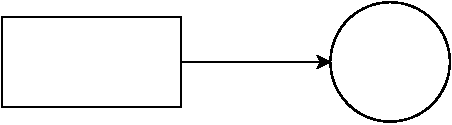
\includegraphics[width=\textwidth,keepaspectratio]{sample}
    \caption[Short sample caption.]{Longer caption that  and shows below the figure.\label{fig:sample}}
\end{figure}
%
Lorem ipsum dolor sit amet, consectetur adipiscing elit.
Mauris sed ipsum risus.
Nulla aliquet quis quam sed eleifend.
Donec rutrum, dolor id vulputate pharetra, nulla tortor laoreet nisl,
pellentesque dapibus velit dolor suscipit purus.
Phasellus vitae eleifend sem.
Integer ultricies ex in neque pellentesque, vitae facilisis orci aliquam.
In pellentesque mollis turpis, eu tristique lacus eleifend nec.
Vestibulum orci neque, rhoncus vitae convallis eu, suscipit quis dui.
Nulla libero elit, porta sit amet sagittis vel, placerat sit amet tortor.
Aliquam hendrerit dolor sit amet sollicitudin ornare.
Aliquam placerat sodales est, in vestibulum nisl efficitur in.
Nulla venenatis aliquam sem, at volutpat nisl pellentesque eleifend.
Praesent vitae euismod nulla, eget vehicula turpis.
Duis quis tellus vitae nisi tempus tincidunt.

\section{Literature Review}%
\label{sec:literature_review}

Vivamus sit amet orci erat.
Morbi eleifend velit purus, sed gravida metus ullamcorper sed.
Aliquam sit amet interdum nulla, in aliquam diam.
Aliquam non libero tortor.
Nulla imperdiet dolor vel justo semper, ut efficitur enim varius.
Donec ultrices odio id orci fringilla tristique.
Ut fringilla nec felis a finibus.
Sed a felis sed odio elementum porta a ac nisl.
Curabitur suscipit, sem et facilisis tempus, nisl elit vestibulum eros, in
varius dolor enim vitae ante.
Vestibulum ante ipsum primis in faucibus orci luctus et ultrices posuere cubilia
curae; Nullam condimentum tempor consectetur.
Aliquam non porta nisi.
Proin molestie tincidunt tellus, id varius nibh finibus eget.

Vestibulum et neque erat.
Curabitur metus velit, dictum non vehicula vitae, sodales sed purus.
In mattis a mauris nec imperdiet.
Duis volutpat mi eget egestas placerat.
Vivamus non purus erat.
Cras quis egestas libero.
Sed id diam at enim vehicula porttitor.

Mauris tincidunt elementum porttitor.
Curabitur eu elit et metus luctus ultrices.
Aenean varius orci in turpis consectetur efficitur.
Quisque lacinia sagittis pharetra.
Aliquam efficitur aliquam arcu, vel ullamcorper tortor volutpat nec.
Curabitur sit amet semper tortor.
Vestibulum ante ipsum primis in faucibus orci luctus et ultrices posuere cubilia
curae; Cras at leo aliquet, porta mauris nec, pharetra augue.
Nam volutpat eu urna in ullamcorper.
Aliquam ultrices condimentum odio id eleifend.
Mauris tellus felis, mattis et pellentesque ac, laoreet vitae eros.
Aliquam at nisl lorem.
Quisque consequat ligula nec tellus ornare eleifend.

\section{Instructions}%
\label{sec:instructions}

This sentence refers to Section~\ref{sec:literature_review}, as an example of
how to do cross-referencing.
Equation~\eqref{eq:emc} shows one of the most famous equations.
%
\begin{equation}
    \label{eq:emc}
    e = mc^2
\end{equation}
%
An example of how to create multiple equations, where they all align is given
below.
%
\begin{align}
    e & = mc^2          \\
    m & = \frac{e}{c^2}
\end{align}

\section{Inserting references}%
\label{sec:inserting_references}

To insert a reference, the entry must be inserted in the \texttt{references.bib}
file.
The key or unique ID of the entry is then used to refer to it.
\LaTeX{} will automatically number the entry and generate the list of
references.
The paper in~\cite{sample_key} is used as a referencing example.

\section{Inserting acronyms}%
\label{sec:inserting_acronyms_and_glossary_entries}

The \gls{tcp} and \gls{udp} protocols are two layer 4 protocols, used for
demonstrating how to use acronyms.
On the second use of an acronym, only its initials are shown as demonstrated in
the following sentence.
The \gls{tcp} and \gls{udp} protocols are two layer 4 protocols, used for
demonstrating how to use acronyms.

\section{Using glossary terms}%
\label{sec:using_glossary_terms}

Let \gls{G} represent a loop-free directed graph, where \gls{V} and \gls{E}
represent the set of nodes and edges, respectively.

\section{Inserting a table}%
\label{sec:inserting_a_table}

A simple table is shown in Table~\ref{tab:simple}, with a more complex example
given in Table~\ref{tab:complex}.

\begin{table}
    \caption{Simple table example.\label{tab:simple}}
    \centering
    \begin{tblr}{|c|S[table-format=3.2]|c|}
        \hline
        \textbf{Header 1} & \textbf{Header 2} & \textbf{Header 3} \\
        \hline
        1                 & 2.3               & Orange            \\
        2                 & 100.5             & Blue              \\
        3                 & 35.0              & Black             \\
        \hline
    \end{tblr}
\end{table}

\begin{table}
    \centering
    \caption{Complex table example.\label{tab:complex}}
    \begin{tblr}{|Q[m,0.2\textwidth]|Q[m,0.2\textwidth]|Q[m,0.2\textwidth]|Q[m,0.2\textwidth]|}
        \hline
        \SetCell[r=2]{c} Table Head & \SetCell[c=3]{c} Table Column Head & & \\
        \hline
        & Table column subhead 1 & Table column subhead 2 & Table column subhead 3 \\
        \hline
        Item 1 & 2 & 3 & 4 \\
        \hline
        Item 2 & 2 & 3 & 4 \\
        \hline
        Item 3 & 2 & 3 & 4 \\
        \hline
        Item 4 & 2 & 3 & 4 \\
        \hline
    \end{tblr}
\end{table}

\section{Inserting code snippet}%
\label{sec:inserting_code_snippet}

The code snippet in Listing~\ref{lst:python_example} demonstrates a very simple
python program.

\begin{lstlisting}[language=Python,caption=Python example,label={lst:python_example}]
def main() -> None:
    print("Hello World")

if __name__ == "__main__":
    main()
\end{lstlisting}

\section{Inserting theorems, corollaries and lemmas}%
\label{sec:inserting_theorems,_corollaries_and_lemmas}

\begin{theorem}
    Let \(f\) be a function whose derivative exists in every point, then \(f\) is
    a continuous function.
\end{theorem}

\begin{theorem}[Pythagorean theorem]
    \label{pythagorean}
    This is a theorem about right triangles and can be summarised in the next
    equation
    \[ x^2 + y^2 = z^2 \]
\end{theorem}

And a consequence of theorem \ref{pythagorean} is the statement in the next
corollary.

\begin{corollary}
    There's no right rectangle whose sides measure 3cm, 4cm, and 6cm.
\end{corollary}

You can reference theorems such as \ref{pythagorean} when a label is assigned.

\begin{lemma}
    Given two line segments whose lengths are \(a\) and \(b\) respectively there is a
    real number \(r\) such that \(b=ra\).
\end{lemma}

\section{Inserting an algorithm}%
\label{sec:inserting_an_algorithm}

The pseudocode for a basic \gls{ea} using NSGA-II is given in
Algorithm~\ref{alg:evolutionaryAlgorithm}.

\begin{algorithm}
    \caption{Pseudocode for an Evolutionary Algorithm}%
    \label{alg:evolutionaryAlgorithm}
    \begin{algorithmic}
        \State \( \mathcal{P} \) = Population Size
        \State \( \chi \) = Number of Generations
        \State \( \omega \) = Crossover Probability
        \State \( \psi \) = Mutation Probability
        \State
        \State population = GenerateInitialPopulation(\( \mathcal{P} \))
        \For{\( 1, 2, \ldots, \chi \)}
        \State offspring = TournamentSelection(population, \( \mathcal{P} \))
        % Crossover
        \For{\(c_i \in \) offspring, \( i = 1, 3, 5, \ldots, \mathcal{P}\)}
        \State \(z\) = random(0, 1)
        \If{\( z < \omega \)}
        \State Crossover(\( c_i, c_{i+1} \))
        \EndIf
        \EndFor
        % Mutation
        \For{\(c_i \in \) offspring}
        \State \(z\) = random(0, 1)
        \If{\( z < \psi \)}
        \State Mutate(\( c_i \))
        \EndIf
        \EndFor
        % Calculate fitness
        \State CalculatePopulationFitness(offspring)
        % Update population size
        \State population = NSGA-II([population + offspring], \(\mathcal{P}\))
        \EndFor
    \end{algorithmic}
\end{algorithm}


\chapter{Introduction}
\label{chp:introduction}

The \acrlong{vqa} problem --- which is a computer vision-language task whereby a system, given a question in the presence of an image, can predict an answer to the question \cite{agrawal_vqa_2016} --- has been leading up to a new problem: \acrfull{vcr}.
The \acrshort{vcr} problem extends the \acrshort{vqa} problem through the complexity of the questions being asked, which require more knowledge and insight to answer than is otherwise immediately apparent in a given image \cite{zellers_recognition_2019}.
Datasets are available for both tasks, and there are numerous \gls{ml} models which have been trained for both tasks.

A class of \gls{ml} models targetting \gls{vqa} tasks known as `compositional models'\cite{andreas_neural_2016} have proven to perform well on \gls{vqa} datasets\cite{fishandi_neural_2023}.
Such performance is attributed to the nature of their design whereby multiple smaller \gls{ml} modules are used to divide and conquer the steps for solving a \gls{vqa} task.
To further explore the use of compositional models in such tasks, we will be looking towards taking an existing model and adapting it to solve tasks that require \gls{vcr}.

While any compositional model could have been chosen for this work, the below characteristics were established to choose one model:

\begin{itemize}\label{list:reasons_for_nmn}
    \item The source code for the model and its distribution are available by the original authors along with steps for reproducing their results.
    \item The architecture of the model is such that each step taken to solve a \gls{vqa} task is performed in a sequential manner which can be viewed at each individual step and should therefore be easier to interpret when compared to other non-compositional models.
          This same behaviour can also be ported to \gls{vcr} tasks which should allow for better exploration of model performance on the task.
    \item The modular nature of the model architecture means future work can expand on its ability to solve \gls{vcr} tasks without necessitating a complete redesign to the model architecture.
    \item The chosen model is fully differentiable, meaning it can be trained without reinforcement learning or supervision of any kind (such as expert layouts) and produce comparable performance to models trained with layout supervision.
\end{itemize}

With the above in mind, the below objectives were established:

\begin{itemize}\label{list:list_of_objectives}
    \item Obtain a working copy of the model.
    \item Confirm the model operates as intended by training it on \gls{vqa} and produce accuracy results matching those published by the model authors (within a reasonable margin).
    \item Modify the model to be able to train and evaluate on the \gls{vcr} dataset.
    \item Perform experiments on the model to test whether certain modifications will produce better results or not.
    \item Following an analysis of its performance, outline future work that may expand upon the findings.
\end{itemize}

This study will begin with a review of the literature available, covering the datasets available for these task types, the models which target these datasets, and a discussion of which model best meets the above criteria for use in this study.
Following the literature review is the methodology of how this model is set up to run on the \gls{vcr} dataset, including what experiments will be run.
The results of these experiments will be explored along with a qualitative analysis of how the model performance compared to other \gls{vcr} models covered in the literature review.
To conclude, a retrospective and discussion of future work will be presented.

\chapter{Literature review}
\label{chp:literature_review}

For this work, we will be exploring a subset of neural AI models know as compositional neural network models.
We will select model of this type by exploring and discussing 3 such models, choosing one with which to proceed.
We will also explore the datasets used by the models down below, determining the characteristics of the datasets and their strengths.

\graphicspath{{content/chapters/literature_review/choosing_the_compositional_model/figures}}

\section{Compositional Model Review}
\label{sec:choosing_the_compositional_model}

In this section, we will be exploring three compositional models that have been considered for this study.

Each subsequent model builds upon the works of the former, adopting a more modular and understandable approach for solving \gls{vqa} tasks while also achieving better performance.

\subsection{Neural Module Network}
\label{subsec:neural_module_network}

The \gls{nmn} model\cite{andreas_neural_2016} is an attention-based compositional model which makes use of an array of \gls{nn} modules to solve \gls{vqa} tasks.
When given an image-question pair, it predicts an answer to the question using the following procedure:

\begin{itemize}\label{list:nmn_procedure}
    \item The image and question are preprocessed, extracting their visual and textual features respectively.
    \item The image features, the question text and the question features are fed to the model as inputs.
    \item A new layout of \gls{nn} modules is created (see Figure~\ref{fig:nmn_overview} for an example) by the question parser.
    \item The image features are inputted to each module, computing the output for each module.
    \item The text features are fed to an \acrshort{lstm}. Based on the input features, the outputs of only a specific set of the \gls{nn} modules will also be fed into the \acrshort{lstm}.
    \item The \gls{lstm} and layout outputs are averaged together to produce a final classification prediction as the answer to the input question.
\end{itemize}

\begin{figure}[htbp]
    \centering
    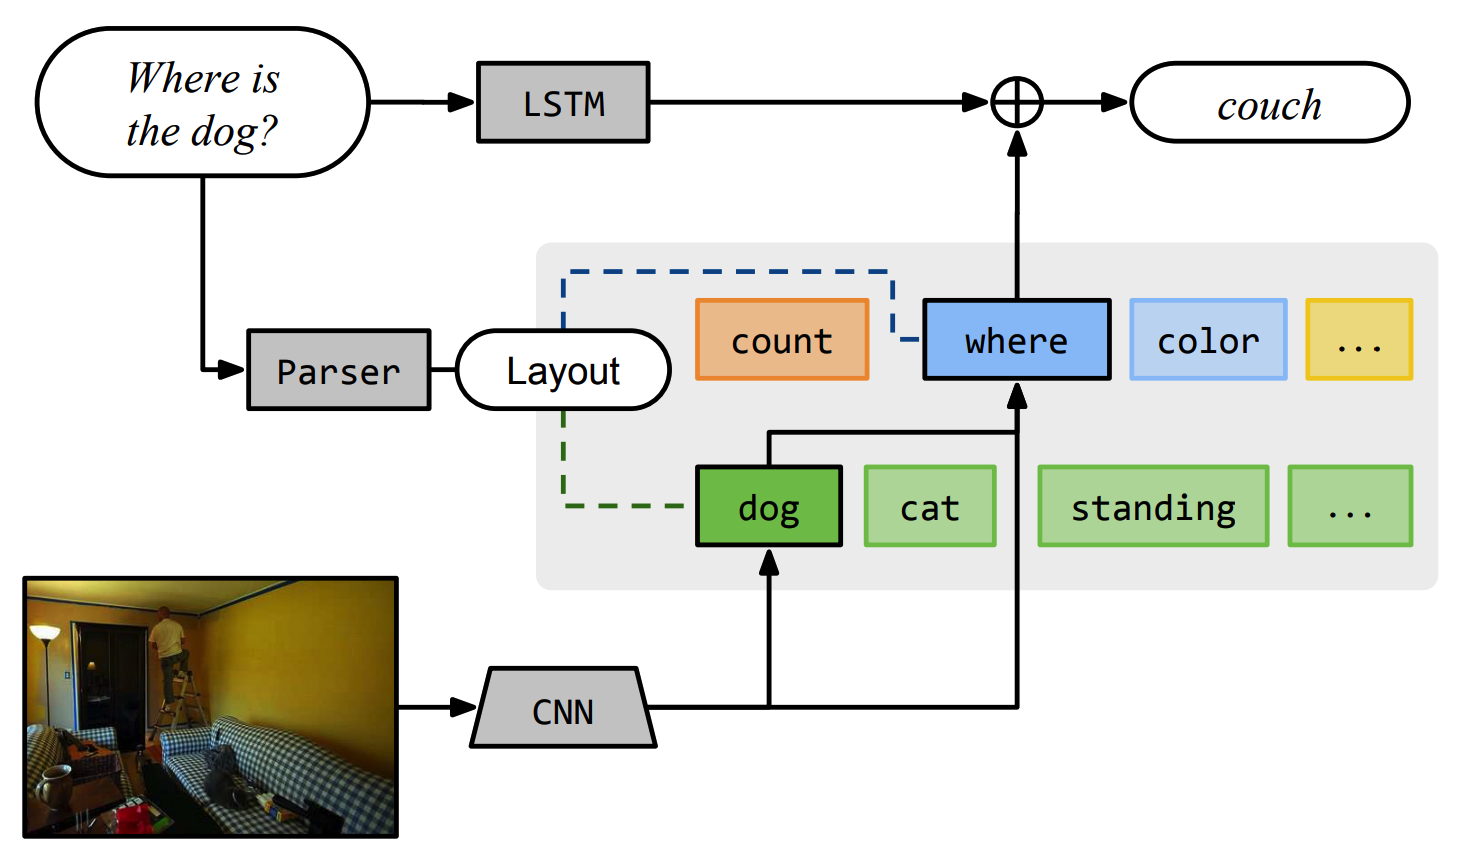
\includegraphics[width=.75\textwidth,keepaspectratio]{nmn_overview}
    \captionsource(\acrshort{nmn} Overview){How an \acrshort{nmn} predicts answers to a \acrshort{vqa} task. \label{fig:nmn_overview}}{\citeauthor{andreas_deep_2016}\cite{andreas_deep_2016}}
\end{figure}

Each module in the \gls{nmn} is described in the format \texttt{type[instance](arg1, ...)}, where \texttt{type} denotes the type of operation performed by the module (eg. \texttt{attend} will search for an object in the image) and \texttt{instance} identifies the module amongst other modules of the same type (eg. \texttt{attend[pillow]} identifies an \texttt{attend} module that looks for \texttt{pillow} objects in the image).
Arguments such as instance or type weights, or other argument types, are shared by the modules.
The paper introduced five module types for its \gls{nmn} model which are given in Table~\ref{tab:nmn_module_list}.

\begin{table}
    \captionsource(\acrshort{nmn} module list){\acrshort{nmn} module types and example uses.\label{tab:nmn_module_list}}{\citeauthor{andreas_neural_2016}\cite{andreas_neural_2016}}
    \centering
    \begin{tblr}{|c|c|c|c|}
        \hline
        \textbf{Module Name} & \textbf{Module label} & \textbf{Inputs \rightarrow Output} & \textbf{Example}          \\
        \hline
        Attention            & \texttt{attend}       & Img \rightarrow Att                & \texttt{attend[ladder]}   \\
        Re-Attention         & \texttt{re-attend}    & Att \rightarrow Att                & \texttt{re-attend[right]} \\
        Combination          & \texttt{combine}      & Att, Att \rightarrow Att           & \texttt{combine[include]} \\
        Classification       & \texttt{classify}     & Img, Att \rightarrow Lbl           & \texttt{classify[colour]} \\
        Measurement          & \texttt{measure}      & Att \rightarrow Lbl                & \texttt{measure[count]}   \\
        \hline
    \end{tblr}
\end{table}

\begin{figure}[htbp]
    \centering
    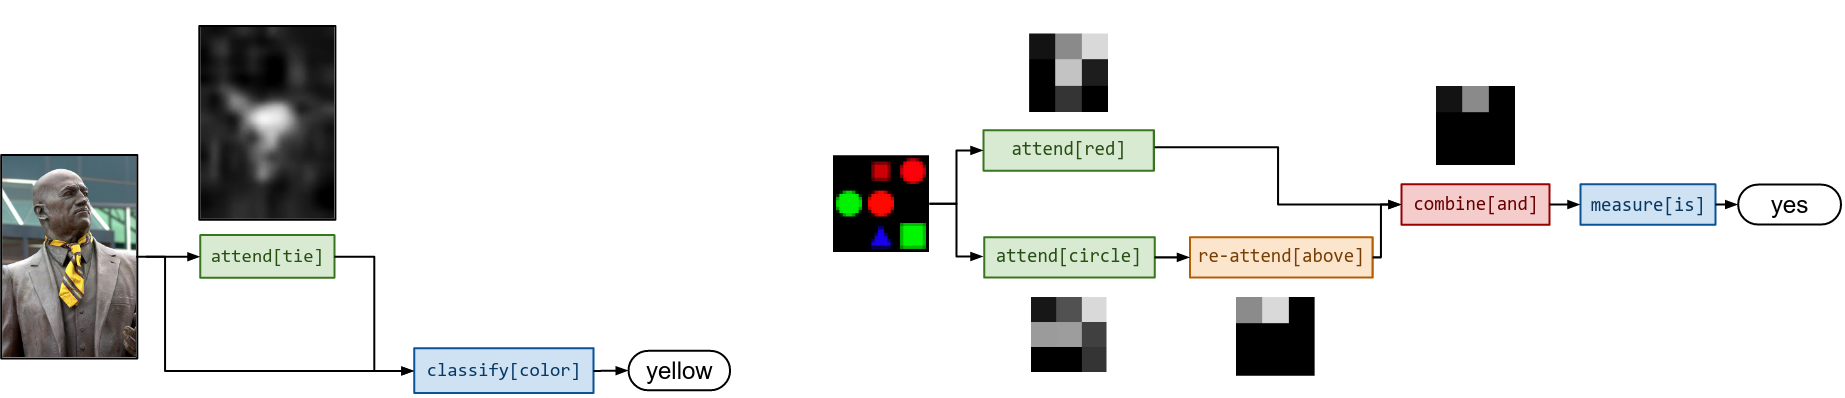
\includegraphics[width=\textwidth,keepaspectratio]{nmn_question_layout}
    \captionsource(\acrshort{nmn} layout construction){Example \acrshort{vqa} tasks being broken down by the \acrshort{nmn}. \textbf{Left:} Question: What colour is his tie? \textbf{Right:} Is there a red shape above a circle? \label{fig:nmn_question_layout}}{\citeauthor{andreas_deep_2016}\cite{andreas_deep_2016}}
\end{figure}

With the module instances prepared, the \gls{nmn} model now needs to know which module instances are required for each question.
To solve this, each question is converted into a layout, which identifies the modules required to answer the question.
To obtain these layouts, each question is first parsed using the Stanford Parser \cite{klein_accurate_2003}, a tool which uses a pre-trained language model to output standardised representations of the questions using the Universal Representations v1 format \cite{nivre_universal_2016}.
These representations are then simplified and converted into tokens which represent the module types and instances supported by the \gls{nmn} (for example: the question \texttt{"What is the colour of the cat left of the truck?"} could be converted into \texttt{"classify[colour](attend[cat](re-attend[left](attend(truck))))}").

While the above provides the model with a solid approach to predicting the answer, it is still susceptible to errors due to overlooked grammatical cues in the question (for example: \texttt{"What is swimming?"} versus \texttt{"What are swimming?"}; both questions denote the answer is something that's swimming, but the second question indicates a plural answer which cannot be represented or conveyed by the layouts protocol established above).
To solve this, the \gls{nmn} uses a \acrlong{lstm} question encoder to detect such cues, and combines its output with the output of the modules.
This effectively gives the final output of the model, the predicted answer to the image-question pair.

\begin{algorithm}
    \captionsource(Pseudocode of \acrshort{nmn} solving \acrshort{vqa} task){A simplified pseudocode of how \acrshort{nmn} solves a \acrshort{vqa} task, from layout construction, to answer prediction.}{Original work written for this study}\label{alg:nmn_solving_pseudocode}
    \begin{algorithmic}[1]
        \State $img_o$ = raw image data \Comment{Original image}
        \State $q_o$ = "What colour is his tie?" \Comment{Original question}
        \State $img_f$ = GetImgFeatures($img_o$) \Comment{Convert to feature map}
        \State $q_{rep}$ = GetUDRepresentation($q_o$) \Comment{Get a Universal Dependency representation}
        \State $q_{func}$ = MapToFunctions($q_{rep}$) \Comment{"What colour is his tie" \rightarrow "colour(tie)"}
        \State $q_l$ = "" \Comment{Final network layout.}
        \ForAll{$w \in q_{func}$} \Comment{First "colour", then "tie"}
        \If{IsRoot($w$)}
        \State PushAnswerNode($q_l$, $w$) \Comment{Either `measure' or `classify' node}
        \ElsIf{IsLeaf($w$)}
        \State PushAttendNode($q_l$, $w$) \Comment{Always an `Attend' node}
        \Else
        \State PushReAttentionNode($q_l$, $w$) \Comment{Either `reattend' or `combine' node}
        \EndIf
        \EndFor
        \State \Comment{$q_l$ is now "classify[colour](attend[tie])"}
        \State $a_{qe}$ = QEncoderPredictAnswer($q_o$) \Comment{Predict answer using \gls{lstm}}
        \State $a_l$ = LayoutPredictAnswer($q_l$) \Comment{Predict answer using layout and modules}
        \State \Comment{Get geometric mean of both predictions (layout-generated and \gls{lstm}-generated)}
        \State $a_{final}$ = $\sqrt[{2}]{a_{qe}a_{l}}$ \Comment{Final answer prediction.}
    \end{algorithmic}
\end{algorithm}

\clearpage
\subsection{End-to-End Module Networks}
\label{subsec:n2nmn}

Building on the \acrshort{nmn} as an attention-compositional neural network, \citeauthor{hu_learning_2017} introduced \acrfull{n2nmn} as an \acrshort{nmn}-based model with an improved layout policy and network assembly \cite{hu_learning_2017} (See Figure~\ref{fig:n2nmn_overview}).

\begin{figure}[htbp]
    \centering
    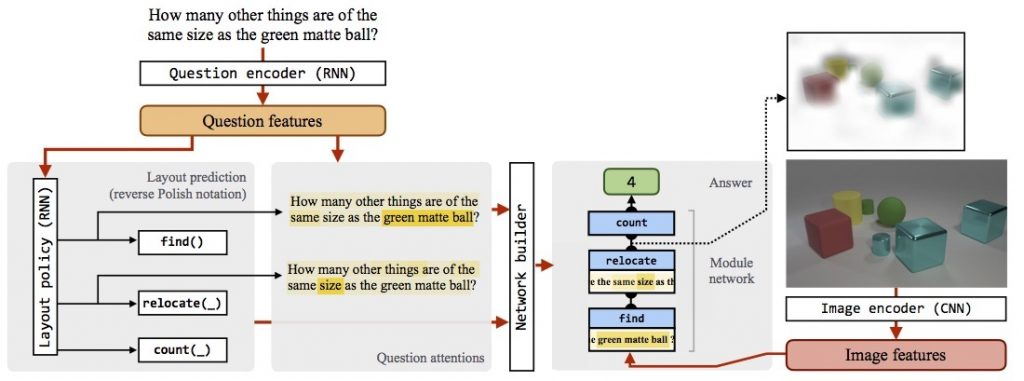
\includegraphics[width=\textwidth,keepaspectratio]{n2nmn_overview}
    \captionsource(\acrshort{n2nmn} model overview){The topology of the \acrshort{n2nmn} model, focusing on its approach to question representation and network layout assembly. \label{fig:n2nmn_overview}}{\url{https://ronghanghu.com/n2nmn/}}
\end{figure}

Similar to \acrshort{nmn}, \acrshort{n2nmn} uses neural modules which take one or two attention maps as input (depending on the module type) and outputs either another attention map or a probability distribution over the possible answers.
Aside from the given input maps, a module-specific textual vector --- obtained from the question being solved --- is also made available at runtime.
This textual vector is created by obtaining an attention map from word embeddings of each word in the question.
With this, a layout expression is created from which the \acrshort{n2nmn} is able to dynamically construct the modules needed using these textual vectors — as shown in Figure~\ref{fig:n2nmn_overview} — without relying on multiple separate, hard-coded module instances as is the case in the \acrshort{nmn} model.
Figure~\ref{fig:n2nmn_layout_breakdown} illustrates how a question is parsed into a solvable layout.

\begin{figure}[htbp]
    \centering
    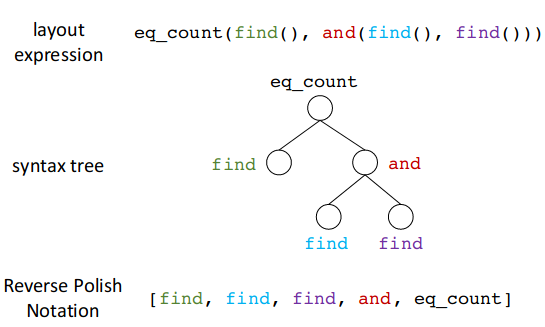
\includegraphics[width=.75\linewidth,keepaspectratio]{n2nmn_rpp}
    \captionsource(\acrshort{n2nmn} using \acrshort{rpp}){How \acrshort{n2nmn} constructs its layout policies using an \acrshort{rpp} sequence of module tokens. \label{fig:n2nmn_rpp}}{\citeauthor{hu_learning_2017}\cite{hu_learning_2017}}
\end{figure}

\begin{figure}[htbp]
    \centering
    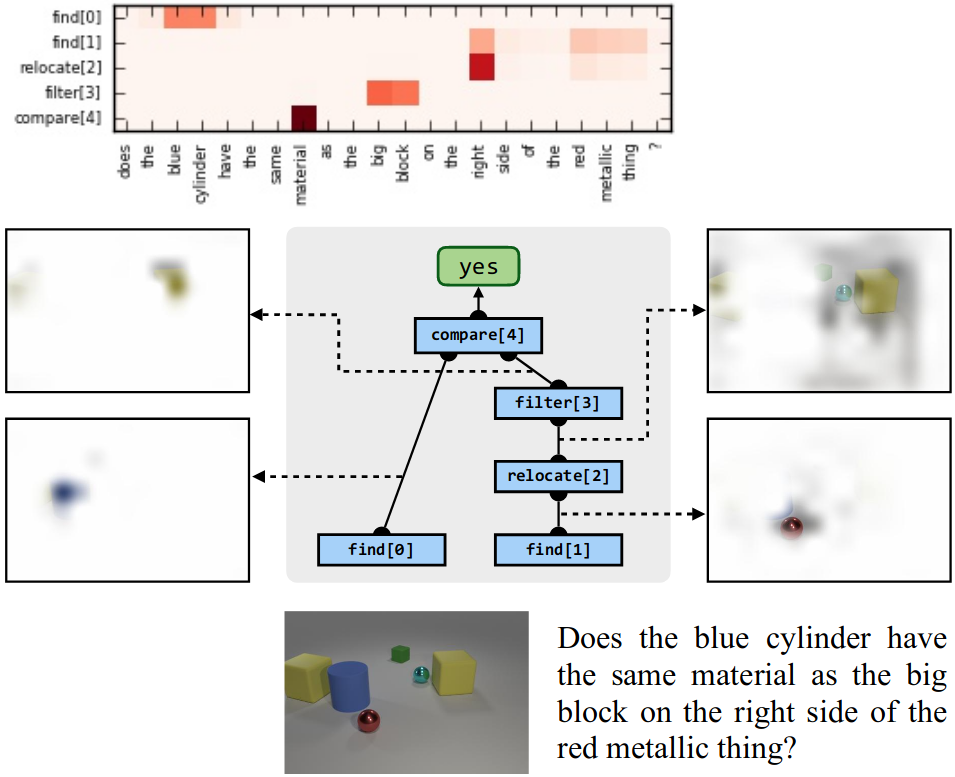
\includegraphics[width=.75\textwidth,keepaspectratio]{n2nmn_layout_breakdown}
    \captionsource(\acrshort{n2nmn} layout construction){A sample breakdown of a \acrshort{vqa} image-question pair, the textual attention for the question, the modules being called and their sequence, and the attentions being produced at each step.\label{fig:n2nmn_layout_breakdown}}{\citeauthor{hu_learning_2017}\cite{hu_learning_2017}}
\end{figure}

The layout expression is then converted into a sequence of module tokens using \acrlong{rpp} as shown in Figure~\ref{fig:n2nmn_rpp}. This has the benefit of representing the solution to predicting the answer as a series of smaller \acrshort{vqa} tasks.
The sequence is then parsed through an attentional \gls{rnn} \cite{bahdanau_neural_2016}. First, all words in the question are embedded into word vectors which are then fed into a multi-layer \gls{lstm}, outputting the encoded question as a vector of equal length.
An \acrshort{lstm} decoder then generates an attention map for the given encoder output and input words.
With this, a distribution of all possible layouts for the question can be predicted.
To narrow this down to the final layout, the model uses a beam search to select the best layout available from the distribution. From this, the final network is assembled.

During training, the layout policy and module parameters are jointly trained, using Adam for parameter optimisation\cite{kingma_adam_2017}, and a loss function over the output answer scores to optimise these parameters.
Due to the layout policy being a discrete training problem, the loss function is not fully differentiable and does not allow for training with full back-propagation.
To circumvent this, those parts which are fully differentiable are trained with back-propagation, while those parts that aren't are trained using a policy gradient method optimised for reinforcement learning.

To optimise training of the layout policy, behavioural cloning is used to significantly reduce the starting loss of the model.
This is done by pre-training the layout policy against a previously-trained layout policy that gives viable performance (referred to as the expert policy).
Once trained, a suitable starting set of parameters are available to the sequence-to-sequence \gls{rnn} and the neural modules.
To avoid biasing of model performance on test sets, expert policies are only used when training on training sets.

\clearpage
\subsection{Stack Neural Module Network}
\label{subsec:stack_neural_module_network}

The \gls{n2nmn} model improved upon the original \gls{nmn}, but can still be improved further in ways that leverage its sequence-based architecture.
Succeeding the \gls{n2nmn} in performance and readability is the \gls{snmn} model, published by \citeauthor{hu_explainable_2019}\cite{hu_explainable_2019}.
The \gls{snmn} architecture is similar to that of \gls{n2nmn} with the exception of how its layouts are selected; whereas the \gls{n2nmn} layout policy selected a discrete set of modules in a layout, the \gls{snmn} layout controller uses a 'soft layout' where all modules are activated and their weighted outputs are averaged (See Figure~\ref{fig:snmn_overview}). The difference in layouts means the \gls{snmn} is fully-differentiable and trainable with back-propagation.

\begin{figure}[htbp]
    \centering
    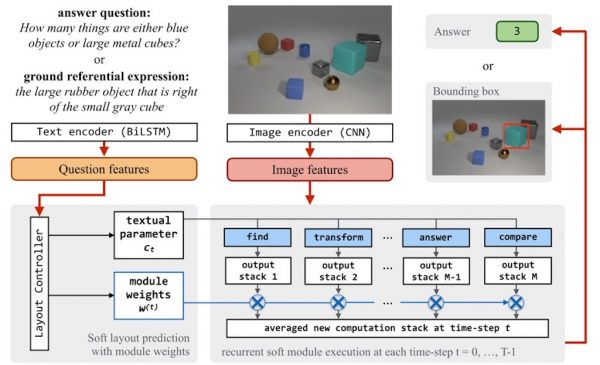
\includegraphics[width=.75\textwidth,keepaspectratio]{snmn_overview}
    \captionsource(\acrshort{snmn} model overview){The topology of the \acrshort{snmn} model and how it solves \acrshort{vqa} and \acrshort{ref} tasks. \label{fig:snmn_overview}}{\url{https://ronghanghu.com/snmn/}}
\end{figure}

The layout controller first encodes the input token sequence representing the question into a textual attention mask sequence representing the question by using a bi-directional \gls{lstm}.
The controller then uses an \acrshort{mlp} to predict a softmaxed attention vector containing a weight for each neural module in the model; this will be the soft layout.
In addition to the soft layout, a textual attention vector is then predicted for each token in the question sequence and used to predict the textual parameter which will be inputted to each module in the network.
The layout controller unrolls itself across all time-steps, repeating the above steps to produce a soft layout, textual parameter, and textual attention vector for each time-step.

\begin{table}
    \centering
    \begin{tblr}{|c|c|c|}
        \hline
        \textbf{Module Name} & \textbf{Inputs \rightarrow Output} & \textbf{Example}             \\
        \hline
        \texttt{Find}        & (None) \rightarrow Att             & \texttt{Find[`chair']()}     \\
        \texttt{Transform}   & Att \rightarrow Att                & \texttt{Transform[`left']()} \\
        \texttt{And}         & Att, Att \rightarrow Att           & Used internally              \\
        \texttt{Or}          & Att, Att \rightarrow Att           & Used internally              \\
        \texttt{Filter}      & Att \rightarrow Att                & \texttt{Filter[`blue']()}    \\
        \texttt{Scene}       & (None) \rightarrow Att             & Used internally              \\
        \texttt{Answer}      & Att \rightarrow Ans                & \texttt{Answer[`exist']()}   \\
        \texttt{Compare}     & Att, Att \rightarrow Att           & \texttt{Compare[`more']()}   \\
        \texttt{NoOp}        & (None) \rightarrow (None)          & Used internally              \\
        \hline
    \end{tblr}
    \captionsource(\acrshort{snmn} module list){\acrshort{snmn} module types and example uses. Some modules are only used internally, or are used as part of the implementation of other modules.\label{tab:snmn_module_list}}{\citeauthor{hu_explainable_2019}\cite{hu_explainable_2019}}
\end{table}

Regarding modules, the \gls{snmn} uses the same module definitions as \gls{n2nmn} but simplified in implementation in some cases (See Table~\ref{tab:snmn_module_list} for a list of all implemented modules).
The main differences between the two implementations is that \gls{snmn} uses a single \texttt{Compare} module for comparison operations and an \texttt{Answer} module for tasks such as measuring or describing.
A \texttt{NoOp} module is also implemented which performs no computation or contribution to the predicted answer, but serves to pad out layouts should they finish before reaching the expected layout size.

Due to the input data requirements of some of the modules, the model needs to be able to provide data from one time-step to a module in a future time-step.
One example case being in \texttt{Compare(Find(), Transform(Find()))}, where the \texttt{Compare()} module needs to know the outputs of both the \texttt{Find()} module and \texttt{Transform()} module which were both executed in separate time-steps.
To address this, a memory stack is used to store outputs from intermediate neural modules where each module can then pop and push data onto the stack as needed.
The stack can store a pre-configured number of fixed-dimension vectors in its memory, while a one-hot vector - the same length as the stack - serves as the stack pointer.
The stack is designed to store image attention maps which are equal in size to the image feature maps.
Modules will then pop as many attention maps as needed and then push their output (if its an attention map) back onto the stack for other modules to use.
The model implements differentiable push and pop operations for manipulating the stack and its stack pointer.

When the model prepares to execute a layout, it begins by initialising the stack and setting the stack pointer to the 1st stack element.
From each time-step after initialisation, every module in the model is executed and popping any needed attention from the stack and pushing back onto the stack.
The result of each module is averaged together to produce a new stack representing the final state of that time-step, and the same averaging is performed on the stack pointer to indicate the top-most element at the end of the time-step.
The final output of the model is determined by averaging the weighted answer \glspl{logit} across all output modules (see Table~\ref{tab:snmn_module_list}) across all time-steps, and summing them to produce a final output \gls{logit}.

\subsection{Model comparison}
\label{subsec:models_comparison}

To discuss and compare the models discussed in Sections~\ref{subsec:neural_module_network} to~\ref{subsec:stack_neural_module_network}, we will be focusing on their performance across the \textit{SHAPES}, \textit{\gls{vqa}}, and \textit{CLEVR} datasets, discussing and elaborating on the performance metrics presented in Table~\ref{tab:model_performance_vqa}.
We will then follow up by highlighting the limitations of each model, and conclude by looking into how easy it is to understand the steps taken by each model to produce the results.

\begin{table}
    \centering
    \begin{tblr}{|l|c|c|c|c|}
        \hline
        \textbf{Model}                       & \textbf{SHAPES} & \textbf{CLEVR}              & \textbf{VQAv1}  & \textbf{VQAv2} \\
        \hline
        \gls{nmn}\cite{andreas_deep_2016}    & 90.6            & 72.1\cite{hu_learning_2017} & 55.1            & -              \\
        \gls{n2nmn}\cite{hu_learning_2017}   & \textbf{100.0}  & 83.7                        & 64.9 (test-dev) & 63.3           \\
        \gls{snmn}\cite{hu_explainable_2019} & -               & \textbf{96.5}               & \textbf{66.0}   & 64.0           \\
        \hline
    \end{tblr}
    \captionsource(\acrshort{vqa} model performance across the \acrshort{vqa} datasets.)
    {Comparison of models across the 3 \acrshort{vqa} datasets discussed. Results are measured in percentage accuracy (\%) and obtained from the highest-scoring run with all performance optimisations (such as expert layout) enabled. \label{tab:model_performance_vqa}}
    {Aggregated from their respective publications\cite{andreas_neural_2016,hu_learning_2017,hu_explainable_2019}.}
\end{table}

Both \gls{nmn} and \gls{n2nmn} performed well on the \textit{SHAPES} dataset, scoring 90.6\% and 100\% respectively.
While the images themselves are not complex at all - being only low-resolution images of 3-coloured 2d shapes - it served as a benchmark for testing the dynamics of a model's layout-construction.
The questions are also yes/no questions meaning most of the performance may be carried by the models final stage which could be performing guesswork on the text of the question.
\gls{snmn} was not tested on this dataset so its performance is not known, but could be assumed to be on-par with \gls{n2nmn} given the similarity in module implementation.

While the \gls{n2nmn} and \gls{snmn} both achieve scores of 83.7\% and 96.5\% on the \textit{CLEVR} dataset respectively, the \gls{nmn} model was not tested on the dataset at the time of its publishing.
Despite this, it was modified to use the expert layout of the \gls{n2nmn} model so it would be able to train and test on the \textit{CLEVR} dataset, with which it was able to score 72.1\%\cite{hu_learning_2017}.
% The \textit{CLEVR} dataset is arguably a more suitable dataset for testing layout-construction than \textit{SHAPES} on account of it featuring the same complexity of questions, having more complex 3d scenes, and featuring many more question-answer sets.

On the \textit{\gls{vqa}v1} dataset, \gls{nmn}, \gls{n2nmn}, and \gls{snmn} achieved test scores of 55.1\%, 64.9\%, and 66\%, respectively. Aside from those results, \gls{n2nmn} and \gls{snmn} were also tested on \gls{vqa}v2 and scored 63.3\% and 64.0\% respectively. Even when tested on natural images, the \gls{snmn} model remains effective, narrowly surpassing the \gls{n2nmn}.

Despite the performance of the \gls{nmn}, there are limitations concerning its ability to answer yes/no questions; as was suggested by \citeauthor{andreas_deep_2016}\cite{andreas_deep_2016}, the model seems to suffer from overfitting when training with yes/no questions.
Aside from this, the model uses hard-coded textual parameters which lead to measurably worse performance in the CLEVR dataset.
This problem does not occur in \gls{n2nmn} since the modules use soft-attention module parameters instead of hard-coded textual parameters.
Additionally, the \gls{n2nmn} seems to learn additional optimisations regarding how it attends to the image (for example: in Figure~\ref{fig:n2nmn_layout_breakdown}, the layout policy seems to `coordinate' two \texttt{find} modules so that one looks to the 'right side of the red metallic thing' while the other looks to the left to try and find the 'red metallic thing').

The main drawback to the \gls{n2nmn} is its inability to use back propagation during training, instead relying on end-to-end training using reinforcement learning.
This limitation is addressed in the \gls{snmn} model, which is able to use back propagation during training thanks to its fully-differentiable layout controller and stack memory structure.
The \gls{snmn} model also shares the same optimisations seen in \gls{n2nmn} of composing a future time-step parameter into the current attention to optimise future time-steps.
Additionally, the \gls{snmn} model produces more human-interpretable results than the other models, and is supported by an experiment which compares the \gls{snmn} model to a more closely-integrated model known as MAC\cite{hudson_compositional_2018} using human evaluators\cite{hu_explainable_2019}.
The model itself shared a very similar approach of using sequential time-steps with textual and visual parameters at each step, but does not use modular networks like the discussed models (see Chapter~\ref{subsec:mac_network} for further details on its implementation).
While the \gls{snmn} model was found to be more understandable and logically-predictable by human evaluators, its performance in the \gls{vqa} dataset was worse (by about 2\%) compared to the MAC model which was the state-of-the-art at the time\cite{hu_explainable_2019}.

When examining each of these models for ease of inclusion in this project, all models are open-source, with their code-bases being released by the original authors.
The original \gls{nmn} model however, is discouraged for use by the original author who favours the newer \gls{n2nmn} model for being easier to set up and better performing\footnote{See \url{https://github.com/jacobandreas/nmn2/blob/master/README.md}}.
Building upon this, the \gls{n2nmn} and \gls{snmn} both share strong similarities in implementation, general architecture, and aims, with the main differences being that the \gls{snmn} uses a different memory structure and modified layout controller.
Aside from those, it also uses more recent versions of their dependencies which will help with the development given the expected \acrshort{gpu} driver requirements for the specified dependency versions are no longer publicly available.
Both these models use this legacy version so ultimately both would require the same rewrite if done.
As a result of the reasons above, the benefits outlined in the discussion of results,
and the ease of predictability of the model for human users who do not know the implementations of the model, the \gls{snmn} model was chosen for this study.

\clearpage
\subsection{Recognition to Cognition}
\label{subsec:recognition_to_cognition}

Having discussed and explored the above \gls{vqa} models, we will now explore two \gls{vcr} models to explore the differences between the \gls{vqa} models reviewed in Sections~\ref{subsec:neural_module_network} to~\ref{subsec:stack_neural_module_network} and these \gls{vcr} ones.
The first \gls{vcr} model chosen is the \gls{r2c} model\cite{zellers_recognition_2019}, introduced alongside the formal \gls{vcr} task declaration and the \gls{vcr} dataset\cite{zellers_recognition_2019}.
The model a different architecture to the compositional models discussed, instead using the following steps to produce its predictions: \textbf{ground}, \textbf{contextualise}, then \textbf{reason}.

\begin{figure}[htbp]
    \centering
    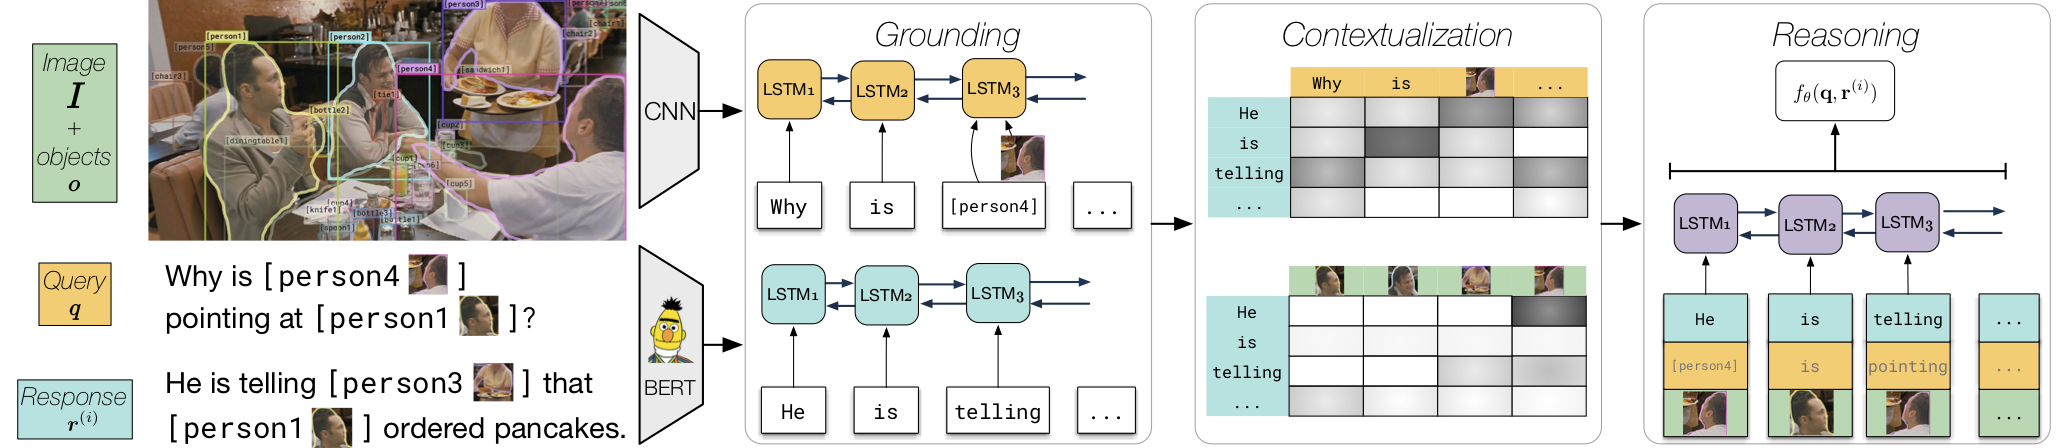
\includegraphics[width=\textwidth,keepaspectratio]{r2c_architecture_overview}
    \captionsource(\acrshort{r2c} model overview){Basic overview of the \acrshort{r2c} model and how it solves a \acrshort{vcr} task. \label{fig:r2c_architecture_overview}}{\url{https://github.com/rowanz/r2c/}}
\end{figure}

All image features are extracted using ResNet-50\cite{he_deep_2015} while language representations of the questions and responses are obtained using BERT\cite{devlin_bert_2019}.
The model is trained to reduce the multi-class cross entropy between the prediction of each response for the question, and the correct-most response.

When given a question-response pair, the model begins by \textbf{grounding} the question and response, by locating the objects in the image which are referenced.
By doing so, it derives the meaning of the question and the intention of each answer and rationale.
The grounding module begins by learning an image-language representation for the given tokens, which it shares for the question and responses (since they share the same vocabulary and tags).
Using this representation, the textual features of the question and responses are obtained.
The \gls{resnet}-generated object features are then combined with each object label's embedding to produce a shared hidden representation.
This shared hidden representation, combining both image and textual features, is fed into a \gls{bilstm} to produce the final outputs of the grounding module.

The outputs of the grounding module are then \textbf{contextualised} using the contextualiser module.
This performs a cross-multiplied softmax between the question, response, and object attentions to obtain the final contextualised representation of the question and the responses.

Finally, \textbf{reasoning} is performed by the model inside its reasoning module.
This is composed of a bidirectional \gls{lstm} which uses the contextualised representation of the question, object attentions, and responses, as input.
The output is then concatenated with the question and answer representations at each timestep for better gradient control by the loss function.
The final concatenated sequence is max-pooled, where an \gls{mlp} predicts a \gls{logit} representing confidence in the question-response pair.

\subsection{Merlot-Reserve}
\label{subsec:merlot_reserve}

\begin{figure}[htbp]
    \centering
    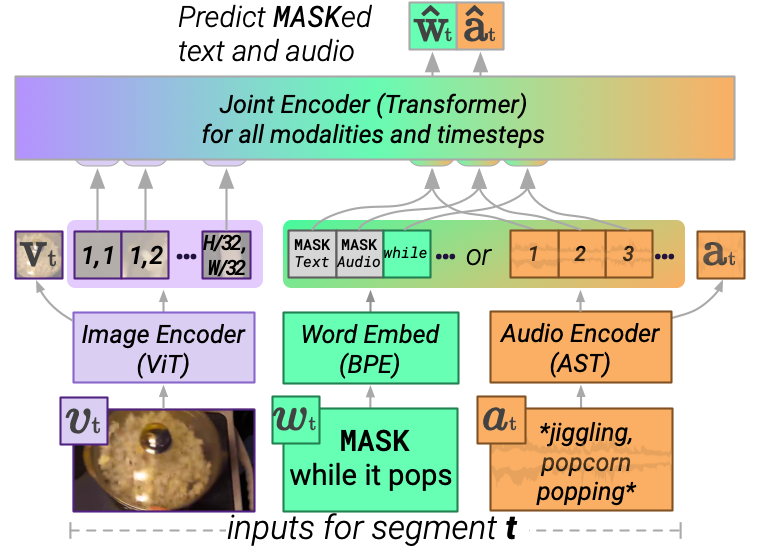
\includegraphics[width=.75\textwidth,keepaspectratio]{merlot_reserve_model}
    \captionsource(MERLOT-RESERVE model overview){An overview of the MERLOT-RESERVE model. Of particular note is it's ability to train using audio data unlike any previously-covered model. \label{fig:merlot_reserve_model_overview}}{\citeauthor{zellers_merlot_2022}\cite{zellers_merlot_2022}}
\end{figure}

To conclude, one final model which can perform \gls{vcr} tasks will be explored.
The model in question is MERLOT-RESERVE, another \gls{vcr} model by Zellers that can train on images, and either text or audio \cite{zellers_merlot_2022}.
The model is transformer-based, unlike previously-explored models which are \gls{rnn}-based, and uses a joint encoder to combine both encoded image data and word embeddings into a final prediction.
The word embeddings are composed using a \gls{bpe} embedding table which creates embedding from a sequence of subword embeddings unlike others such as BERT or GLOVE which generate whole-token embeddings\cite{heinzerling_bpemb_2018}.
It also introduces a novel method for training called Contrastive Span Training, where the model is trained on a dataset of video-audio-subtitle entries to produce a generalised model that can be finetuned onto \gls{vcr} and other tasks\cite{zellers_merlot_2022}.
To train, each video is paired with a text/audio sequence that has a region masked out and the model must predict the correct audio or text that matches the masked as closely as possible.
The result is a model that achieved state-of-the-art results at its time\cite{zellers_merlot_2022} and still ranks among the top 15 scoring \gls{vcr} models at the time of writing this study\footnote[1]{\url{https://visualcommonsense.com/leaderboard/}}.

\clearpage
\graphicspath{{content/chapters/literature_review/datasets/figures}}

\section{Datasets}
\label{sec:datasets}

There are 4 \gls{vqa} datasets that will be explored and discussed in this section. As the strengths and scopes of each one are discussed, a final dataset will be discussed which goes a step beyond \gls{vqa}.

\subsection{SHAPES}
\label{subsec:shapes_dataset}

\begin{figure}[htbp]
    \centering
    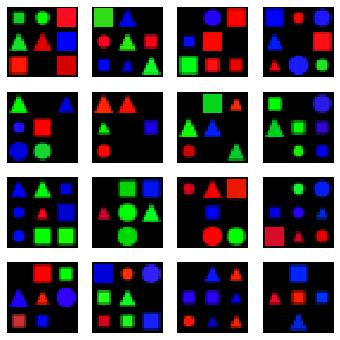
\includegraphics[width=.35\textwidth,keepaspectratio]{shapes_example_images}
    \captionsource(Example SHAPES entries){Example images from the SHAPES dataset. \label{fig:shapes_example_images}}{\url{https://paperswithcode.com/dataset/shapes-1}}
\end{figure}

The SHAPES dataset is a \gls{vqa} dataset introduced by \citeauthor{andreas_deep_2016} \cite{andreas_deep_2016} consisting of synthetic images designed to test the layout construction of compositional neural models.
Each image-question pair consists of a simple image with 9 possible locations for objects and a number of visible shapes in each image.
These shapes are simple uniform shapes (triangles, squares, or circles) with only a difference in color  (red, green, or blue) to distinguish them (see Figure~\ref{fig:shapes_example_images}).
The questions on the other hand are complex with each question containing up to 4 different object attributes, types, or relationships.
The questions found in the dataset can be deliberately false (such as \texttt{Is a red shape blue?} or \texttt{Is the red square a triangle?}) or valid questions (such as \texttt{Is the red object left of a blue triangle a square?}).

\subsection{VQA}
\label{subsec:vqa_dataset}

\begin{figure}[htbp]
    \centering
    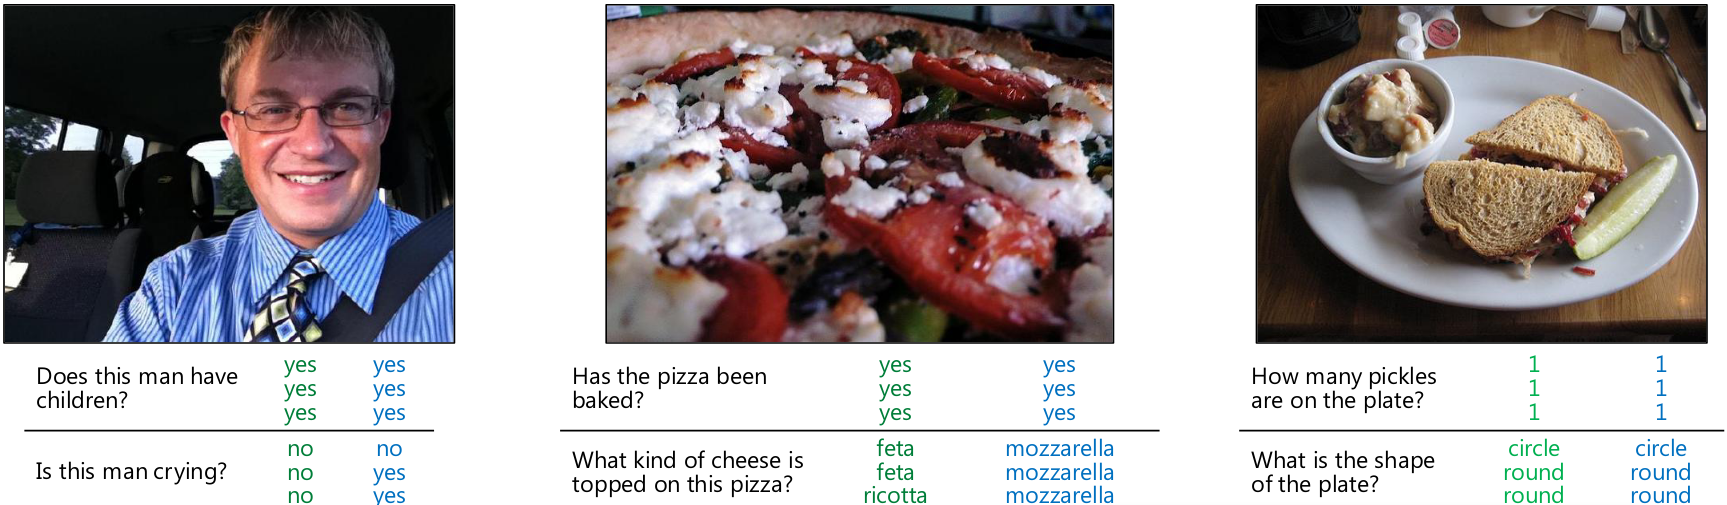
\includegraphics[width=\textwidth,keepaspectratio]{vqa_questions_answers}
    \captionsource(Example \acrshort{vqa} entries){Example images from the \acrshort{vqa} dataset with a question per image and answers. Green answers are valid answers for the given image while blue answers would be valid without the image. Only the green answers are used throughout. \label{fig:vqa_questions_answers}}{\citeauthor{agrawal_vqa_2016}\cite{agrawal_vqa_2016}}
\end{figure}

The VQA dataset \cite{agrawal_vqa_2016} is a natural image dataset composed of 204,721 images, 1,105,904 questions, and 10 acceptable ground truth answers per question.
The images are taken from the COCO image dataset \cite{lin_microsoft_2015} real-life objects, scenarios, and entities, while the questions and answers are supplied by human annotators.
All questions are open-ended, with an array of possble answers to select from and a subset of answers which are possible/correct (See Figure~\ref{fig:vqa_questions_answers} for example image-question pairs with answers).

\subsection{CLEVR}
\label{subsec:clevr_dataset}

\begin{figure}[htbp]
    \centering
    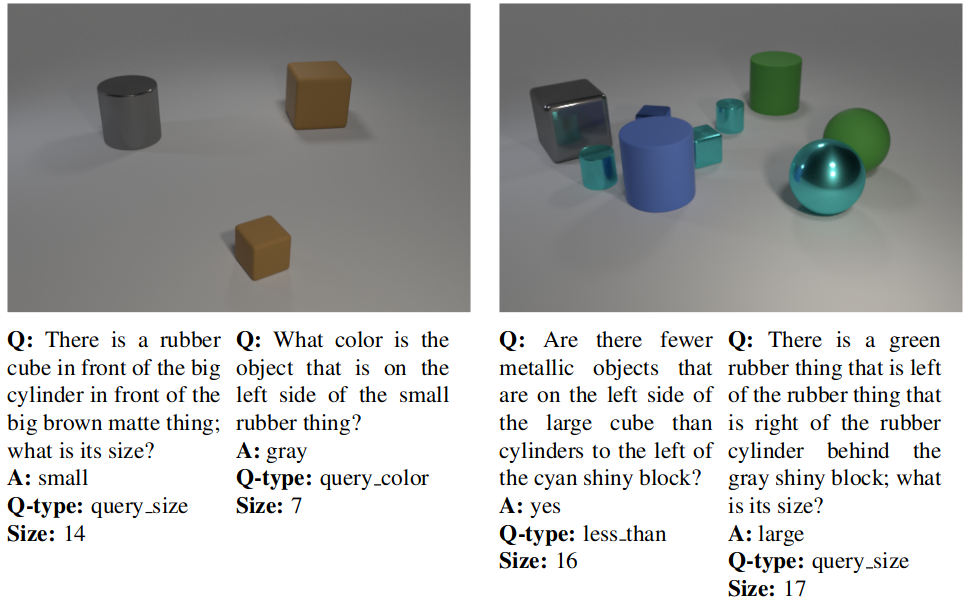
\includegraphics[width=\textwidth,keepaspectratio]{clevr_questions_answers}
    \captionsource(Example CLEVR entries){Example images from the CLEVR dataset with a question per image and the correct answer. Additionally, there's also the type of question included (such as classifying the size or colour) and the size of the datasets included expert layout/program. \label{fig:clevr_questions_answers}}{\citeauthor{johnson_clevr_2016}\cite{johnson_clevr_2016}}
\end{figure}

The CLEVR dataset \cite{johnson_clevr_2016} is a \gls{vqa} dataset designed to test and benchmark compositional \gls{vqa} models.
Similar to the \hyperref[subsec:shapes_dataset]{SHAPES} dataset, each image is a blank scene with any number of 3d shapes which can differ in shape, colour, size, and material (being either shiny metal, or matte rubber).

Questions vary in the type of answer expected (such as counting, yes/no, object attributes), and are diverse in structure, length, query types used through and relationship queries (see Figure~\ref{fig:clevr_questions_answers}).
In total, CLEVR contains 100,000 images and 864,968 questions, with a single correct answer being given per question.

\subsection{GQA}
\label{subsec:gqa_dataset}

\begin{figure}[htbp]
    \centering
    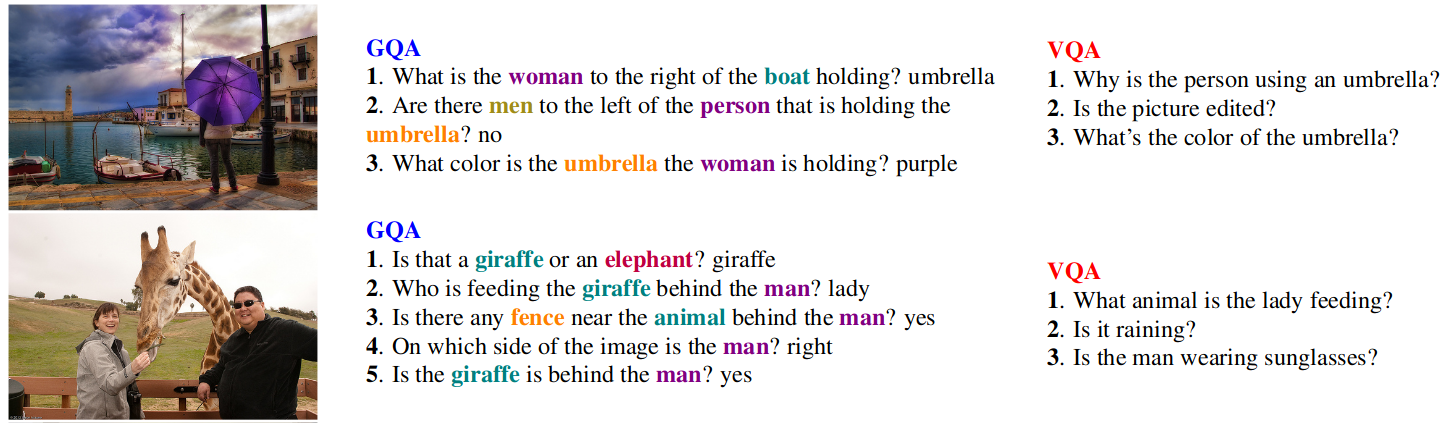
\includegraphics[width=\textwidth,keepaspectratio]{gqa_vqa_questions_comparison}
    \captionsource(Example GQA questions){Comparison of questions from both GQA (left) and \gls{vqa} (right) datasets for the same image. The GQA questions feature greater emphasis on object relations and compositionality than the \gls{vqa} questions are which are comparatively vague or ambiguous. \label{fig:gqa_and_vqa_questions_compared}}{\citeauthor{hudson_gqa_2019}\cite{hudson_gqa_2019}}
\end{figure}

The \gls{gqa} dataset was introduced by \citeauthor{hudson_gqa_2019}\cite{hudson_gqa_2019} as a collection of highly compositional questions to better train compositional \gls{vqa} models.
The dataset contains over 110,000 images --- sourced from various image datasets --- and over 22,000,000 questions.
\todo[inline]{Elaborate further?}

Alongside each image is a scene-graph which describes the objects in the image, object relations, and image location details.
Each question in the training set describes a program in the form of semantic steps which --- if executed by a training model --- would lead to a greater probability of predicting the correct answer.
These steps mimic how a person would apply reasoning to a question to provide an answer to it and should therefore train a model how to perform such reasoning.

\subsection{VCR}
\label{subsec:vcr_dataset}

The VCR dataset \cite{zellers_recognition_2019} was introduced alongside the formalisation of the \gls{vcr} task as the first dataset of the kind.
The images in the dataset are largely frames from movies or clips, and are chosen because of the inherent context supplied by the movies that's required to understand the images.
Because of this, each question in the dataset is about something present within context that cannot be immediately recognised by simple object detection and will thus require additional cognition to answer.
The questions, answers, and rationales, also make use of bounding boxes to identify each person/object of interest, and uses their box names when referring to them (see Figure~\ref{fig:vcr_question_answer} for an example of how these are used).
Aside from answering each question, there is also a further task of providing rationale behind the given answer.
In this subtask, the model would have to produce its reasoning for predicting the initial answer by predicting the correct rationale for the correct answer.
There is only one correct answer and one correct rationale per-question.
There are 3 modes of question-answering available by the dataset as broken down below:

\begin{itemize}\label{list:vcr_task_types}
    \item (Q \rightarrow A): Predict the correct answer for a given image and question.
    \item (QA \rightarrow R): Predict the correct rationale for the given answer to a given question and image.
    \item (Q \rightarrow AR): Using only the image and question, predict both the correct answer and correct rationale.
\end{itemize}

\begin{figure}[htbp]
    \centering
    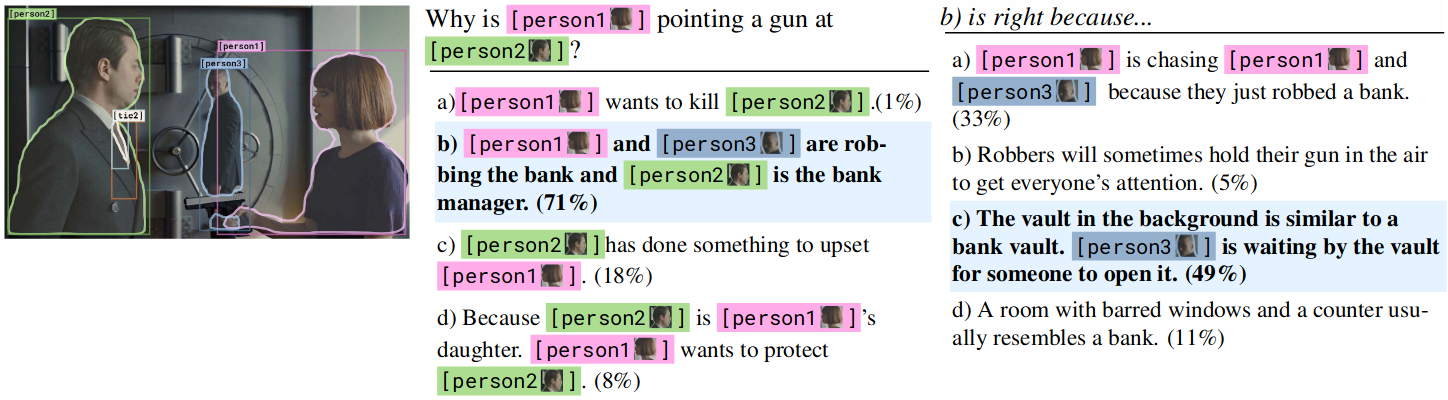
\includegraphics[width=\textwidth,keepaspectratio]{vcr_question_answer}
    \captionsource(Example \acrshort{vcr} entry){Example \acrshort{vcr} task from the \acrshort{vcr} dataset. The text shows how each object in the image is highlighted by the provided bounding box metadata. \label{fig:vcr_question_answer}}{\citeauthor{zellers_recognition_2019}\cite{zellers_recognition_2019}}
\end{figure}

In total, there are 99,904 images, 264,720 questions, 1,058,880 answers, and 1,058,880 rationale.
Each image in the dataset comes with many question files, each containing a question about the image with one correct answer and one correct rationale per-question.
A further 3 incorrect answers and 3 incorrect rationale are included with the correct ones, which are correct answers or rationale to one other question in the dataset (in other words, each answer/rationale is correct at least once across all questions in the dataset).
Each question file (outside of the test fold) specifies the correct answers for the question, and the 'correctness' of each answer.
% Not all information about the file is discussed (such as the ids of each question relative to the image or fold it belongs to).
Each image is accompanied with a metadata json file containing the dimensions of the image, the class names of the objects present (eg. person, car, dog, etc), and the bounding boxes and polygons identifying each object in the image.
All bounding boxes and polygons were generated using the Detectron object detection system\cite{Detectron2018}.


\chapter{Methodology}
\label{chp:methodology}

\section{Data preparation}
\label{sec:data_preparation}

Before the model can begin to perform \gls{vqa} tasks, the required data must first be prepared into a format that will be understood by the model.
The procedure below is followed across all datasets trained and tested on, with variations being made depending on the structure of the data.

The images are first pre-processed into a feature-set using a \acrshort{resnet}-152 model \cite{he_deep_2015} --- pre-trained on the ImageNet\footnote{\url{https://www.image-net.org/}} dataset \cite{deng_imagenet_2009} --- which outputs a 7x7x2048-dimension feature map of each image.
The question-answer pairs found in the dataset are processed after the images.
For each question and answer sentence, the sentence is first collected into a single \gls{corpus} for later processing.
The sentence is tokenised into a series of words, numbers, and/or symbols representing the sentence.
Each occurrence of a token in the sequence is recorded into a vocabulary file which keeps track of every token encountered in the dataset.
Each entry in the vocabulary file contains both the token and the number of occurrences of the token in the \gls{corpus}.

The image features, questions, and answers, are then converted into an \gls{imdb} file.
This file contains a record for every \acrshort{vqa} task, for each split of the dataset (training set, validation set if present, and test set).
Each record identifies the image by its feature file.
A question and all relevant answers are saved as both strings and tokenised variants in the record, along with the correct answer for that question.
If the split does not mark the correct answers (such as with the test set), then the correct answer fields are simply omitted.

With the \gls{imdb} files prepared, next would be to prepare the text embeddings for the model.
This is done by converting each token in the vocabulary file into a 300-dimensional word vector following the same procedure as was used by \citeauthor{hu_learning_2017} in their \gls{n2nmn} model \cite{hu_learning_2017}.
For this, a GloVe model \cite{pennington_glove_2014} was trained on the prepared dataset \gls{corpus} and vocabulary --- obtained when preparing the \gls{imdb} files --- to produce a word embeddings file, where each entry belongs to the token on the same line number in the vocabulary file.

\subsection{Preparing for VCR data}
\label{subsec:preparing_the_vcr_data}

There are a number of properties about the dataset that need to be handled when preparing the dataset for processing.
To begin with, each \gls{vcr} task in the dataset is referred to as an `annotation' which links one unique question and several answers and rationales to an image.
Each question, answer, rationale, and image, have a unique annotation index based on the fold and split they're found.
These indices are important as each annotation entry inside the dataset uses these indices to reference which answer/rationale are correct and which image to use.
There is only one correct answer/rationale per-annotation, which is the one unique to that annotation alone - all other wrong answers/rationales in that annotation are copies from other annotations and referenced as such by their indices.
Aside from these, an 'interestingness score' is provided by the annotation authors (not the dataset authors themselves, but the ones to whom the annotation task was outsourced) for each annotation, as a subjective ranking of how interesting the annotation would be.
There's also a 'likelihood score' provided by the annotation authors whereby they assess how likely it is that the question, answer, and rationale given by them actually fit the context of the source movie the annotated image was taken from.
Finally, there's a ranking of each answer and rationale by correctness in descending order, where the correct choice is rank 0, rank 1 would be the first wrong choice, and so on.
For the purpose of this work, both the interestingness score and the likelihood score are ignored and the only correctness considered per-annotation are whether the choice is correct or not.

Aside from the annotations entries, each image in the dataset contains a metadata file, describing the image.
Each file contains the names of object classes found in the image (such as person, car, food, etc).
Aside from the above classes, each object is also identified by a region which can be used to locate the object in the image, and a segmented polygon which highlights of the image.
The model will not use the object regions in the metadata file because it would fall outside the scope of this work.

Like in the previous datasets, the \gls{vcr} dataset is compiled into \gls{imdb} files.
These files contain the same image name, feature path, the question, all answers, and all rationales, for each annotation.
Besides the above, additional preprocessing is done to make the data compatible with the model and also obtain the word embeddings.
The sentences also make reference to the objects described in the image metadata file by pointing to an index.
This is replaced by the object class described in the metadata file to avoid troubles encountered in inferring what object is being referenced by the image (for eg. a sentence like 'What is [1] pointing to?' becomes 'What is \textit{person} pointing to?').
Each token encountered is extracted into a vocabulary file which contains each found token and the total number of occurrences.
Each sentence (question, answer, or rationale) is added to a \gls{corpus} file, which will be used to by GloVe to prepare the word embeddings.
Currently, there is no filtering made when preparing the corpus, so duplicate sentences, whether correct or wrong, are also added.
Additionally, BERT will also be used for generating word embeddings since \citeauthor{zellers_recognition_2019} found that their model performed best for \gls{vcr} when using BERT embeddings\cite{zellers_recognition_2019}.

\section{Model adaptation}
\label{sec:model_adaptation}

For the purposes of this dissertation --- to perform \gls{vcr} tasks using the \gls{snmn} architecture --- several adaptations and modifications were needed to the model.
The \gls{vqa} implementation of the model is used as the base since it most closely matches the \gls{vcr} dataset since both the \gls{vqa} and \gls{vcr} datasets represent plausible real-life settings (the CLEVR implementation, like the dataset, is mainly focused on benchmarking the performance of \gls{vqa} on synthetic images).

\subsection{Layout generator}
\label{subsec:layout_generator}

The biggest difference between the original implementation and the current implementation comes from the \gls{vcr} dataset using single-choice (multiclass) questions instead of open-ended questions with one-word answers.
The original model as a result would only encode the question text and ignore the answer/rationale text completely (see Figure~\ref{fig:base_snmn_input_unit}).
Since the questions are single-choice, the model would need to look at each answer (and rationale) individually, as if it were part of the question text.
To support this, the input unit of model was modified to encode the question, answer, and rationale as input by concatenating their embeddings together into a single encoded vector (see Figure\ref{fig:vcr_snmn_input_unit}).
The input unit would also produce an attention mask that would properly identify the lengths of each input sentence without relying on padding.
Once both the encoding and attention mask are produced, the layout generator proceeds with the same flow as the original model.

\begin{figure}[htbp]
    \centering
    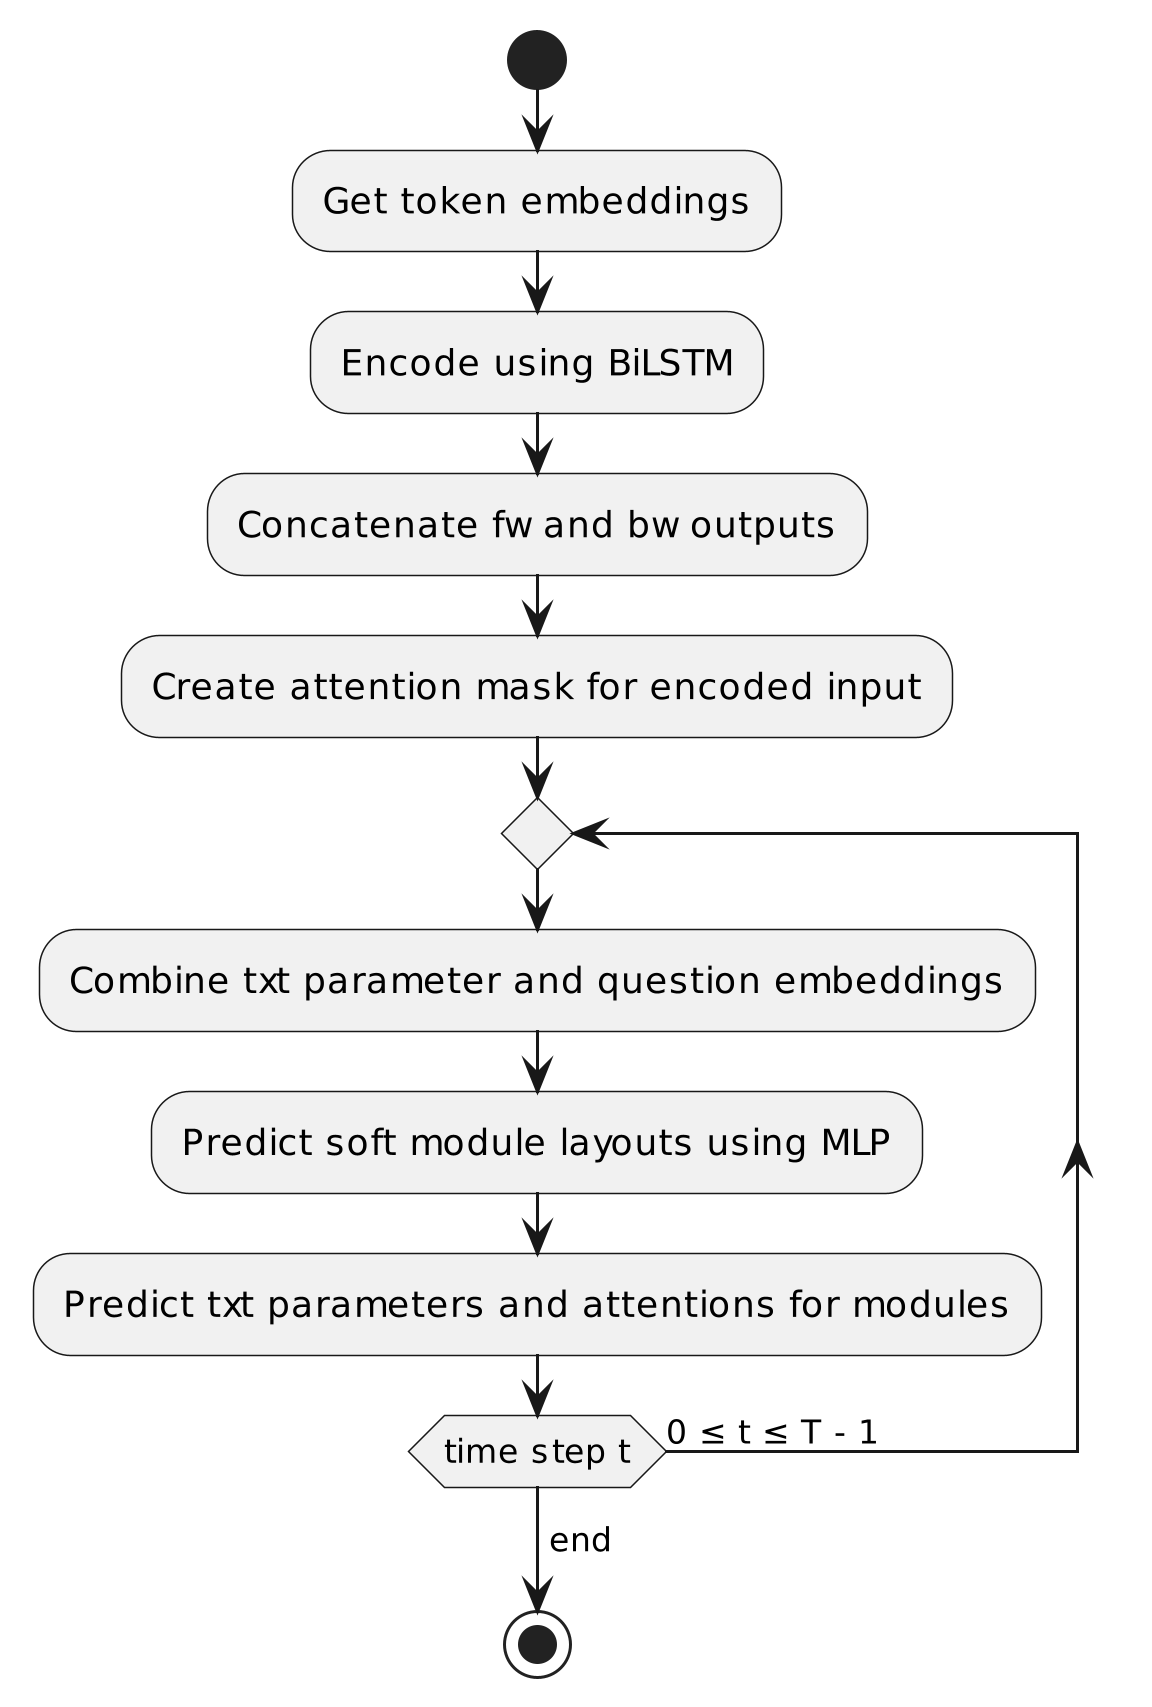
\includegraphics[width=.55\textwidth,keepaspectratio]{content/chapters/methodology/model_adaptation/figures/controller-layout-base-snmn.png}
    \captionsource(Base \gls{snmn} \gls{nas} implementation){Flow diagram of how the \gls{snmn} converts the input question to a layout.\label{fig:base_snmn_input_unit}}{Original diagram prepared for this dissertation}
\end{figure}

\begin{figure}[htbp]
    \centering
    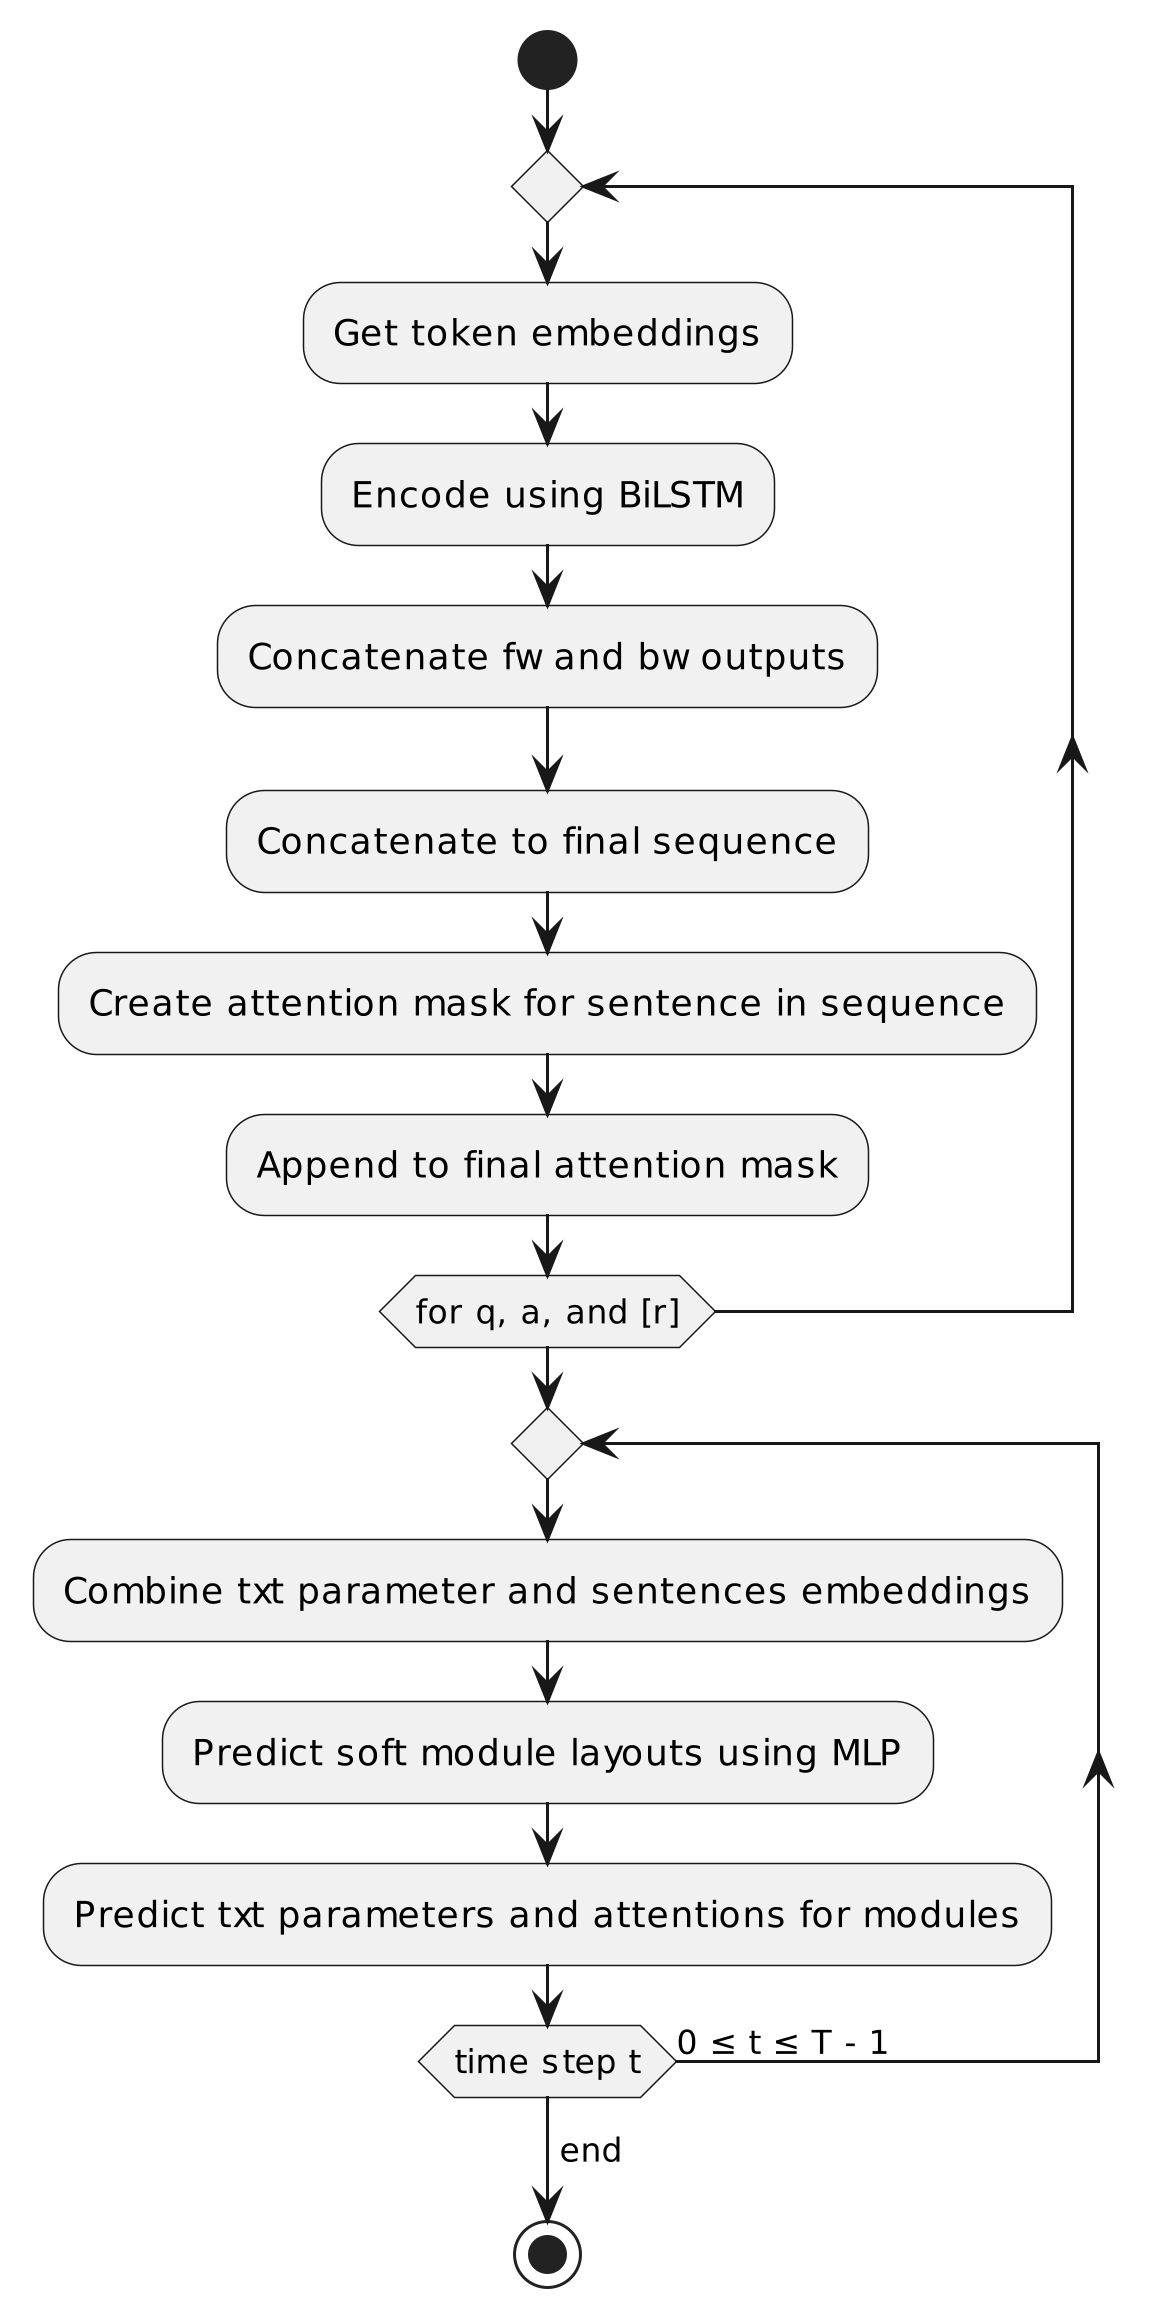
\includegraphics[width=.55\textwidth,keepaspectratio]{content/chapters/methodology/model_adaptation/figures/controller-layout-vcr-snmn.png}
    \captionsource(Modified \gls{snmn} \gls{nas} implementation){Flow diagram of how the \gls{vcr}-adapted \gls{snmn} converts the input question, answer, and rationale to a layout. Note that the rationale is only used when answering \gls{vcr} questions in QAR mode.\label{fig:vcr_snmn_input_unit}}{Original diagram prepared for this dissertation}
\end{figure}

\subsection{Output and loss function}
\label{subsec:output_and_loss_function}

Another problem arising from this question type is that it's incompatible with the original loss function of the program.
The original loss function used a softmax cross-entropy over the whole vocabulary, which is good for multilabel classification (selecting one or more correct choices) but not for multiclass classification (only one correct choice).
The new loss function uses a sigmoid cross-entropy over the prediction \glspl{logit} for each combination of question, answers, and rationales.
In other words, for each \gls{vcr} task with one question, four possible answers, and four possible rationales, the loss function will expect sixteen probability scores, with the score closest to 1 being given to the correct answer and rationale.
To form the input for the loss function, the model is run once for each input combination for the one \gls{vcr} task, a softmax vector is created from the combination of outputs, and used as input for the loss function.


\chapter{Results}
\label{chp:results}

Now that the methodology has been covered, the results of the experiments described in Section~\ref{sec:experiments} will be presented.
A discussion of the results and the challenges encountered will also be given.

\section{Evaluation results}
\label{sec:evaluation-results}

The accuracy results for the experiments can be found in Table~\ref{tab:experiment-results}.
All experiments were carried out by training on the vcr-train set first, then testing against the vcr-eval set.
Each experiment model is trained for up to 75k steps with checkpoints taken at 5k step intervals.
The batch size used is 64 for Q\rightarrow{}A tasks, 16 for QA\rightarrow{}R and Q\rightarrow{}AR using BERT, and 24/32 for QA\rightarrow{}R and Q\rightarrow{}AR using Word2Vec-768 and Word2Vec-300 respectively.

\todo[inline]{Explain why different batch sizes were used (limitations of runtime).}

In every task type, the BERT embeddings model outperformed the other models with GLOVE or Word2Vec embeddings and eaching as high as 63\% in Q\rightarrow{}A tasks.
GLOVE achieved the second-best performance overall with up to 52\% Q\rightarrow{}A, but showing no learning signs in Q\rightarrow{}AR tasks with an avg. accuracy only 0.15\% higher than random guessing.
Word2Vec performend the worst across all tasks and failed to complete the full training course on QAp\rightarrow{}R and Q\rightarrow{}AR tasks.
The results suggest that the contextual embeddings generated by BERT contribute significantly to the model performance (aligning with the results found by \citeauthor{zellers_recognition_2019} where using GLOVE also resulted in worse accuracy\cite{zellers_recognition_2019}).

When performing the QAp\rightarrow{}R tasks, BERT achieved 60\% while GLOVE failed to achieve a meaningfully higher score than random guessing (26\% compared to 25\%) and Word2Vec failed to complete training.
It appears the embeddings BERT produces allow for the model to compensate for possibly embeddings from possibly-incorrect answers.
This would explain why the GLOVE model fails to produce meaningful accuracy because it does not rely on sentence-level context between sentences.


\begin{table}[]
    \begin{threeparttable}
        \begin{tabularx}{\linewidth}{r||cc|ccc|cc}
            \hline
            \multicolumn{8}{c}{Experiment results (vcr-eval)} \\ \hline
             & Q\rightarrow{}A & Q\rightarrow{}A & QA\rightarrow{}R & QA\rightarrow{}R & QAp\rightarrow{}R & Q\rightarrow{}AR & Q\rightarrow{}AR \\
            Wrd Embed. & Shr. & Sep. & Shr. & Sep. & Shr. & Shr & Sep. \\
            Rand Guess & 25\% & 25\% & 25\% & 25\% & 25\% & 6.25\% & 6.25\% \\
            Glove-300 & 52\% & 51\% & 25\% & 47\% & 26\% & 6.4\%\tnote{3} & 6.4\%\tnote{3} \\
            BERT-768 & 63\% & 63\% & 60\%\tnote{3} & 60\%\tnote{3} & 60\%\tnote{3} & 24.7\%\tnote{3} & 24\%\tnote{3} \\
            w2v-300 & 33\%\tnote{1} & 34\% & 25\% & 32\%\tnote{2}\tnote{3} & - & - & - \\
            w2v-768 & 32\%\tnote{1} & 34\% & 25\% & 32\% & - & - & - \\
            \hline
        \end{tabularx}

        \begin{tablenotes}
            \item[1] Problems with loss function resulting in partial training or lack of training.
            \item[2] Training program crashed at least once and had to be resumed from prior checkpoints.
            \item[3] Trained on multi-\gls{gpu} configuration.
        \end{tablenotes}
    \end{threeparttable}
    \captionsource(Evaluation results)
        {Evaluation results from running the model across combinations of different token embeddings, VCR task types, and layout generator configurations. \textit{Shr.} refers to models with a shared \gls{bilstm} while \textit{Sep.} refers to one \gls{bilstm} per input sentence. \label{tab:experiment-results}}
        {Original performance results obtained for this dissertation.}
\end{table}

\todo[inline]{Add discussion on why some experiments are in multi-gpu and some are single-gpu. Include table comparing one of these results.}

\section{Challenges}
\label{sec:experiment-challenges}

Several problems were encountered during training.
The most common error encountered was unstable learning which resulted in NaN loss errors or slow learning.
NaN losses were frequent when training the model using word2vec embeddings and didn't occur at all when using glove or bert.
Slow learning rates were observed during glove and word2vec training, especially with Q\rightarrow{}AR training.
Another factor in getting good predictions was batch size, which was strained by the task size and amount of data involved.
To work around the limited batch size available, training on QA\rightarrow{}R and Q\rightarrow{}AR modes was performed on a multi-gpu setup to allow for increased batch size.
This setup produced better learning rates and prediction performance compared to single-gpu training, at the cost of increased runtime due to the synchronisation overhead of keeping the two gpu models in mirrored.


\printbibliography[title=References]

\appendix{}

\chapter{Generating the input files used by the model}
\label{chp:appendix_a}

Before running the model, the dataset is first prepared into a set of binary tfrecords files.
These files allow for streaming data to the model in a more optimised manner than json-based files.
To prepare these files, the image features are first generated using a \gls{resnet}152 model, with each feature file saved as a tfrecords file.
A script then generates the textual data through the following steps:
\begin{itemize}
    \item Extracting the individual \gls{vcr} entries and sorting them by set.
    \item Record the vocabulary found in all entries and output it to a file.
    \item Compile a corpus file from the entries.
    \item Save the entries into imdb files according to set.
\end{itemize}

The GLOVE word embeddings for the \gls{imdb} files are generated using a script to perform the below steps:
\begin{itemize}
    \item Generate a co-occurrence matrix on the \gls{corpus} and vocabulary files that were previously compiled.
    \item Convert the co-occurrence matrix to a final 300-dimensional embeddings file.
    \item Convert the embeddings into a binary file for loading and parsing by the model at startup.
\end{itemize}

To generate the BERT embeddings files, the existing \gls{r2c} author-provided \gls{vcr} embeddings are downloaded.
They are then extracted into a set tfrecords files according to the set they belong to (train, val, and test).

A script generates the Word2Vec embeddings from the previously-generated vocabulary file.
The script is configurable to determine the model type used for generating the embeddings and the output vector size.

The final dataloader constructs an optimised data pipeline for the model to consume which concurrently loads and prefetches these separate file sources and maps them into the final expected format for the model to train, evaluate, and test itself.

% \chapter{Generating the input files used by the model}
\label{chp:appendix_a}

Before running the model, the dataset is first prepared into a set of binary tfrecords files.
These files allow for streaming data to the model in a more optimised manner than json-based files.
To prepare these files, the image features are first generated using a \gls{resnet}152 model, with each feature file saved as a tfrecords file.
A script then generates the textual data through the following steps:
\begin{itemize}
    \item Extracting the individual \gls{vcr} entries and sorting them by set.
    \item Record the vocabulary found in all entries and output it to a file.
    \item Compile a corpus file from the entries.
    \item Save the entries into imdb files according to set.
\end{itemize}

The GLOVE word embeddings for the \gls{imdb} files are generated using a script to perform the below steps:
\begin{itemize}
    \item Generate a co-occurrence matrix on the \gls{corpus} and vocabulary files that were previously compiled.
    \item Convert the co-occurrence matrix to a final 300-dimensional embeddings file.
    \item Convert the embeddings into a binary file for loading and parsing by the model at startup.
\end{itemize}

To generate the BERT embeddings files, the existing \gls{r2c} author-provided \gls{vcr} embeddings are downloaded.
They are then extracted into a set tfrecords files according to the set they belong to (train, val, and test).

A script generates the Word2Vec embeddings from the previously-generated vocabulary file.
The script is configurable to determine the model type used for generating the embeddings and the output vector size.

The final dataloader constructs an optimised data pipeline for the model to consume which concurrently loads and prefetches these separate file sources and maps them into the final expected format for the model to train, evaluate, and test itself.

% \chapter{Sample B}

Lorem ipsum dolor sit amet, consectetur adipiscing elit.
Mauris sed ipsum risus.
Nulla aliquet quis quam sed eleifend.
Donec rutrum, dolor id vulputate pharetra, nulla tortor laoreet nisl,
pellentesque dapibus velit dolor suscipit purus.
Phasellus vitae eleifend sem.
Integer ultricies ex in neque pellentesque, vitae facilisis orci aliquam.
In pellentesque mollis turpis, eu tristique lacus eleifend nec.
Vestibulum orci neque, rhoncus vitae convallis eu, suscipit quis dui.
Nulla libero elit, porta sit amet sagittis vel, placerat sit amet tortor.
Aliquam hendrerit dolor sit amet sollicitudin ornare.
Aliquam placerat sodales est, in vestibulum nisl efficitur in.
Nulla venenatis aliquam sem, at volutpat nisl pellentesque eleifend.
Praesent vitae euismod nulla, eget vehicula turpis.
Duis quis tellus vitae nisi tempus tincidunt.

Nam quis aliquet nisi, non pharetra ligula.
Phasellus pulvinar mattis neque, nec interdum justo condimentum hendrerit.
Mauris fermentum venenatis faucibus.
Pellentesque egestas eleifend libero, quis placerat ante fermentum et.
Suspendisse accumsan gravida rhoncus.
Vestibulum auctor sodales vehicula.
Pellentesque a urna et elit placerat laoreet a quis turpis.
Morbi ut sem at nunc posuere malesuada vel nec libero.
Nam et urna suscipit, bibendum diam sed, aliquet leo.
Lorem ipsum dolor sit amet, consectetur adipiscing elit.
Ut pretium mauris et nulla malesuada, mattis tristique lectus molestie.
Aenean accumsan iaculis quam, eget varius libero placerat eu.
Fusce mauris justo, vulputate a sollicitudin a, malesuada at est.
Sed ac augue elit.
Maecenas massa lorem, tincidunt vitae neque et, maximus dictum tellus.


\end{document}
